
% Copyright 2007, 2008, 2009 Elsevier Ltd 
% 
% This file is part of the 'Elsarticle Bundle'.
% --------------------------------------------- 
%
% It may be distributed under the conditions of the LaTeX Project Public
% License, either version 1.2 of this license or (at your option) any
% later version.  The latest version of this license is in
%    http://www.latex-project.org/lppl.txt
% and version 1.2 or later is part of all distributions of LaTeX
% version 1999/12/01 or later c.
%
% The list of all files belonging to the 'Elsarticle Bundle' is
% given in the file `manifest.txt'.
%
 
% Template article for Elsevier's document class `elsarticle'
% with harvard style bibliographic references
% SP 2008/03/01
%
%
%
% $Id: elsarticle-template-harv.tex 4 2009-10-24 08:22:58Z rishi $
%
%
%\documentclass[preprint,authoryear,12pt]{elsarticle}
\documentclass[preprint,12pt]{elsarticle}

% Use the option review to obtain double line spacing
%\documentclass[authoryear,preprint,review,12pt]{elsarticle}

% Use the options 1p,twocolumn; 3p; 3p,twocolumn; 5p; or 5p,twocolumn
% for a journal layout:
%\documentclass[final,authoryear,1p,times]{elsarticle}
%\documentclass[final,authoryear,1p,times,twocolumn]{elsarticle}
%\documentclass[final,authoryear,3p,times]{elsarticle}
%\documentclass[final,authoryear,3p,times,twocolumn]{elsarticle}
%\documentclass[final,authoryear,5p,times]{elsarticle}
%\documentclass[final,authoryear,5p,times,twocolumn]{elsarticle}

%% if you use PostScript figures in your article
%% use the gra

%%graphis package for simple commands
%% \usepackage{graphics}
%\usepackage{cases}
%% or use the graphicx package for more complicated commands
\usepackage{graphicx}
%% or use the epsfig package if you prefer to use the old commands
\usepackage{epsfig}
%\usepackage{subfig}
\usepackage{comment}

\usepackage{epstopdf}
\usepackage{pdflscape}
\usepackage{bm}
\usepackage{hyperref,url}
\hypersetup{colorlinks=true, urlcolor=blue, linkcolor=blue, citecolor=red}

%% The amssymb package provides various useful mathematical symbols

\usepackage{amssymb,amsmath,array}
%The amsthm package provides extended theorem environments

\usepackage{amsthm}
\usepackage{graphicx}
%\usepackage{subfigure}
  
%% The lineno packages adds line numbers. Start line numbering with
%% \begin{linenumbers}, end it with \end{linenumbers}. Or switch it on
%% for the whole article with \linenumbers after \end{frontmatter}.
%% \usepackage{lineno}

\usepackage{lscape}

%% natbib.sty is loaded by default. However, natbib options can be
%% provided with \biboptions{...} command. Following options are
%% valid:

%%   round  -  round parentheses are used (default)
%%   square -  square brackets are used   [option]
%%   curly  -  curly braces are used      {option}
%%   angle  -  angle brackets are used    <option>
%%   semicolon  -  multiple citations separated by semi-colon (default)
%%   colon  - same as semicolon, an earlier confusion
%%   comma  -  separated by comma
%%   authoryear - selects author-year citations (default)
%%   numbers-  selects numerical citations
%%   super  -  numerical citations as superscripts
%%   sort   -  sorts multiple citations according to order in ref. list
%%   sort&compress   -  like sort, but also compresses numerical citations
%%   compress - compresses without sorting
%%   longnamesfirst  -  makes first citation full author list
%%
%% \biboptions{longnamesfirst,comma}

% \biboptions{}

\newcommand{\JGnote}[1]{\fbox{\parbox{\textwidth}{ \color{red} JG Note $\Rightarrow$ #1}}}
\newcommand{\KCnote}[1]{\fbox{\parbox{\textwidth}{ \color{black} KC Note $\Rightarrow$ #1}}}
\newcommand{\red}{\textcolor{red}}
\newcommand{\blue}{\textcolor{blue}}
\newcommand{\green}{\textcolor{green}}
\newcommand{\frc}{\displaystyle\frac}
\newcommand{\PN}[2][error]{P$_{#1}$DG-P$_{#2}$}
\newcommand{\PNDG}[2][error]{P$_{#1}$DG-P$_{#2}$DG}
\newcommand{\eg}{{\it e.g., }} 
\newcommand{\ie}{{\it i.e., }}

\journal{Applied Mathematical Modelling}

\begin{document}

\begin{frontmatter}

%% Title, authors and addresses

%% use the tnoteref command within \title for footnotes;
%% use the tnotetext command for the associated footnote;
%% use the fnref command within \author or \address for footnotes;
%% use the fntext command for the associated footnote;
%% use the corref command within \author for corresponding author footnotes;
%% use the cortext command for the associated footnote;
%% use the ead command for the email address,
%% and the form \ead[url] for the home page:
%%
%% \title{Title\tnoteref{label1}}
%% \tnotetext[label1]{}
%% \author{Name\corref{cor1}\fnref{label2}}
%% \ead{email address}
%% \ead[url]{home page}
%% \fntext[label2]{}
%% \cortext[cor1]{}
%% \address{Address\fnref{label3}} 
%% \fntext[label3]{}

  \title{ Numerical Investigation of Stochastic and Determininstic Upscaling Methods for Permeability Fields; Using SVD}
\author[UoA]{Babatunde Lashore} \author[UoA]{J.L.M.A. Gomes}
\cortext[cor1]{Corresponding author.}
\address[UoA]{Mechanics of Fluids, Soils \& Structures Group, School of Engineering, University of Aberdeen, UK}


\begin{abstract}
  BlaBlaBla
\end{abstract}



\begin{keyword} %% keywords here, in the form: keyword \sep keyword
Singular Value Decomposition, SVD\sep Upscaling\sep Model Order Reduction, MOD \sep  Principal Component Spaces \sep Permeability field
\end{keyword}
 
\end{frontmatter}

%%%%%%%%%%%%%%%%%%%%%%%%%%%%%%%%%%%%%%%%%%%%%%%%%%%%%%%%%%%%%%%%%%%%%%%%%%%%%%%%%%%%%%%%%%%%%%%%%%%%%%%%%%%%%%%%%%%%%%%%%%%%%%%%%%%%%%%%%%%%%%%%%%%%%%%%%%%%%%%%%%%%%%%%%%%%%%%%%%%%%%%%%%%%%%%%%%% 
\section{Introduction}\label{section:intro}
Naturally occuring rock formations are inherently heterogeneous, which means that the rock properties such as permeability, pore spaces ({\it i.e.}, porosity) and pore throat vary from point to point, and at different length scales. The heterogeneity of rock formations (studied under the general title of porous media) is relevant in calculations required for understanding transportation and storage of fluids in porous media. This is because the heterogeneous properties are important parameters in the mathematical models used for the aforementioned calculations. Therefore, the representation of these heterogeneous properties is of great importance to the porous media and applied mathematics community as well as the oil and gas industry, the Carbon Capture and Storage (CCS) industry, and waste management industry for whom this has direct application in reservoir management, CO$_2$ transportation and storage in subsurface rocks and remediation of contaminated soil respectively.

Furthermore, due to limitations in computing resources, for simulations with very fine grids it is neither efficient nor possible to obtain exact values of geological properties at all points in the domain (\ie scale problems) \cite{Renard_1997} \cite{miller_1998} \cite{chen_2006}. This is particularly true for large geological domains which span several kilometres. Additionally, it is not possible to obtain reliable and accurate spatial information about geological properties throughout the domain ({\it i.e.}, uncertainty problems). It is possible to overcome these challenges by upscaling. Upscaling techniques solve both problems by replacing discrete geological and fluid property values of detailed high resolution domains with coarse descriptions (low resolution) of these properties \cite{Vereecken_2007}. And upscaling techniques which best preserve the statistical properties and flow dynamics behaviour of the high resolution domain gives the best representation of the heterogeneous property.

There are several upscaling techniques which fall under different categories \cite{Renard_1997, Szymkiewicz_2013, Hasting_2001}, however over the last decade, techniques classed as stochastic have received great attention from academic and industrial porous media communities worldwide \cite{Verwoerd_2009, Ravalec-Dupin_2010, Guilleminot_2012}. One of the reasons for this is because stochastic techniques are robust enough to handle multiphase flow in porous media, and they address scale and uncertainity problems which were previously mentioned.

This work couples stochastic and deterministic upscaling representations of the permeability field to a novel high-order accurate control volume finite element method (CVFEM) (see \cite{Gomes_2017} for further details of the model formulation) so as to investigate statistical properties and multiphase flow behaviour in highly heterogeneous porous media. 

Four upscaling techniques are investigated in this research. The arithmetic and harmonic mean are used to obtain the first two upscaled representation and these two are classed as deterministic techniques. The third is a randomly generated permeability field with a Guassian distribution, prescribed by a probability density function (PDF) which was obtained from a base case ({\it i.e.}, high-resolution mesh with known permeability distribution). The four upscaling technique is the crux of this research, it introduces singular value decomposition (SVD) as a method of upscaling using interpolation within the concept of principal component space to reduce the order of the permeability field.

In section 2, the basic mathematical explanation of SVD and its associated linear algebra properties are presented. The the concept of spaces is explained from the engineer's perspective and also from the mathematician's perspective. The objective of this explanation is to assist both parties in visualizing the relevant spaces and performing the necessary transformation within those spaces. Finally, the section describes model order space reduction for the permeability field within the principal component space. Section 3, starts by describing the high resolution base case on which the four upscaling techniques are modelled. The the simulation run which is similar for all the cases/models is described. A brief summary of the pre-processing step for each of the models is also presented. Section 4 provides the results of for the simulations, Section 5 discusses the results of the simulations and gives further intepretation to the result obtained from the SVD upscaling techniques; and section 6 provides the conclusion.


\section{Singular Value Decomposition, SVD, and its application for reducing the order of a permeability field}






%\section{Acknowledgements}
%Mr William Rad\"unz would like to acknowledge the support from the Brazilian Research Council (CNPq) under the \textit{Science without Borders scholarship programme}. Mr Konstantinos Christou would like to acknowledge the support of the University of Aberdeen - College of Physical Science as well as the Aberdeen Formation Evaluation Society (\textit{AFES} is an SPWLA chapter). 

\clearpage 
%% References with bibTeX database:
\bibliographystyle{elsarticle-harv} 
%\bibliographystyle{elsarticle-num}
%\bibliographystyle{apacite}
\bibliography{references}
  
\clearpage 

\listoftables
\clearpage
%
\begin{landscape}
\begin{table}
  \begin{tabular}{c | c c  c  c  c  c  c  c  c  c  c   c}
    \hline
      {\bf Section} & $\phi$ & VR  & $S^{0}_{w}$ & $S^{0}_{nw}$ & $K_{1}$ & $K_{2}$ & $K_{3}$ & $K_{4}$ & $K_{5}$ & $S_{w,irr}$ & $S_{nw,r}$ & $u^{0}_{w}$ \\ 
    \hline
      \ref{section:results_validation} & 0.2  & 1.0  & 0.0  & 1.0  & 1.0  & 2.5  & N/A  & N/A  & N/A & 0.2  & 0.3 & 1.0 \\
      \ref{section:results_homo_hete}   & 0.2  & 1.0  & 0.0  & 1.0  &  XX  & N/A  & N/A  & N/A  & N/A & 0.2  & 0.3 & XX  \\
                                       & 0.2  & 10.0 & 0.0  & 1.0  &  XX  & N/A  & N/A  & N/A  & N/A & 0.2  & 0.3 & XX  \\
      \hline
   \end{tabular}
   \caption{Sumary of model set-up used in the numerical simulations. Superscript $0$ denotes initial condition. \red{(KOSTAS, PLEASE: 1. DOUBLE CHECK THE K, u and S0 VALUES FROM THE MPML FILES; 2. REPLACE ALL XX; 3. COMPLETE THE TABLE FOR ALL SECTIONS/SIMULATIONS.  $S_{w,irr}$ and $S_{nw,r}$ are the same for all simulations.) }}\label{table:setup}
\end{table}
\end{landscape}
\clearpage

\clearpage  
\listoffigures
\clearpage

%%%%
%%%%  FIGURE 
%%%%
\begin{figure}[h]
\centering
\vbox{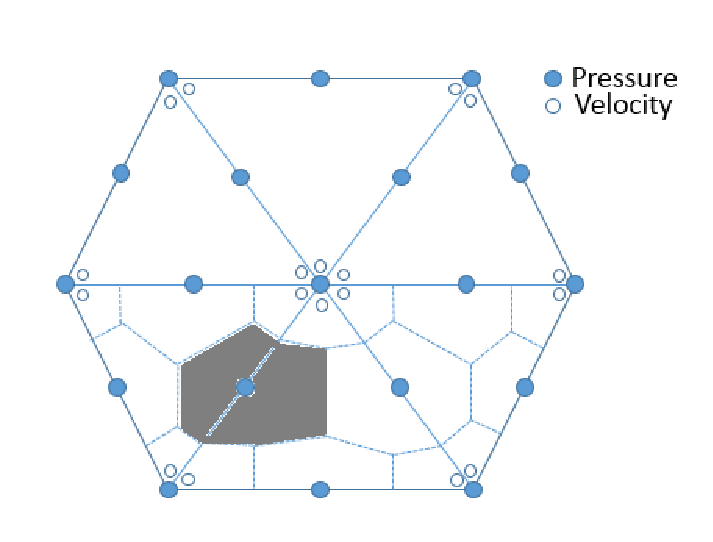
\includegraphics[width=.5\textwidth]{./Pics/P1DGP2.pdf}}
\caption{2D representation of \PN[1]{2} element pairs used in this work. Shaded areas denote control volumes across two contiguous elements. Blue and white circles represent pressure and velocity nodes, respectively.} 
\label{fig:fem_cv}
\end{figure}

\clearpage

%%%%
%%%%  FIGURE
%%%%
\begin{figure}[h]
\centering
\vbox{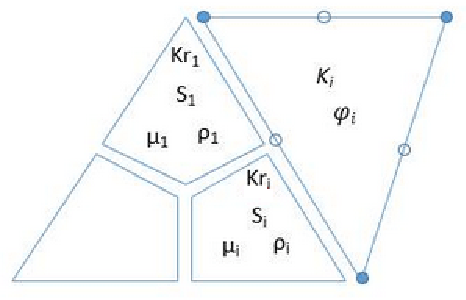
\includegraphics[width=.75\textwidth]{./Pics/element_n.pdf}}
\caption{This is a graphical representation of two different element types. Triangle {\it A} is a representation of the \PN[1]{2} element-pair, whereas triangle {\it B} represents the \PN[1]{1} element-pair. Porosity $\phi_{i}$, permeability {\bf K}$_{i}$, velocity and pressure are primarily represented in FE space whereas scalar fields (such as saturation, density, viscosity etc) are represented in CV space.}
\label{fig:fem_elem}
\end{figure}
\clearpage

%%%%
%%%%  FIGURE 
%%%%
\begin{figure}[h]
\centering
\vbox{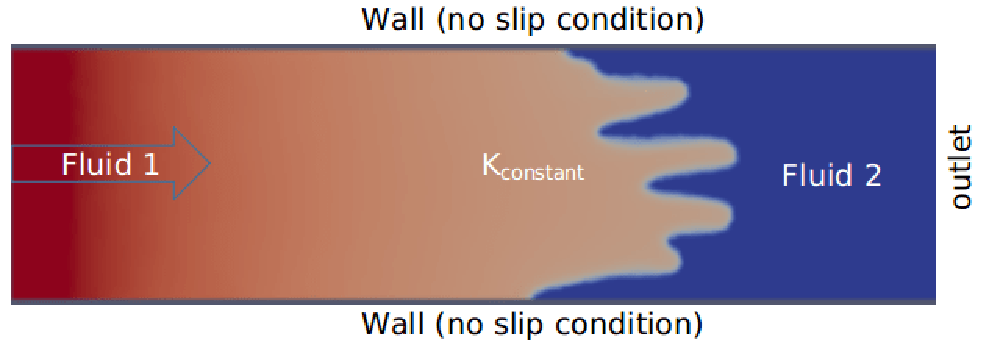
\includegraphics[width=0.75\textwidth]{./Pics/phase_vol_frac_uni_perm_1.pdf}}
\caption{Schematics of formation of flow instabilities during injection of a pure low viscosity fluid (red) into a domain saturated with a second fluid (dark blue). The ratio of viscosity between the two fluids is 5. In this case, the initially piston shape front collapses leading to the formation of several fingers.}
\label{fig:simple_case}
\end{figure}
\clearpage


%%%%
%%%%  FIGURE 
%%%%
\begin{figure}[ht] 
\vbox{
\hbox{\hspace{-0.3cm}
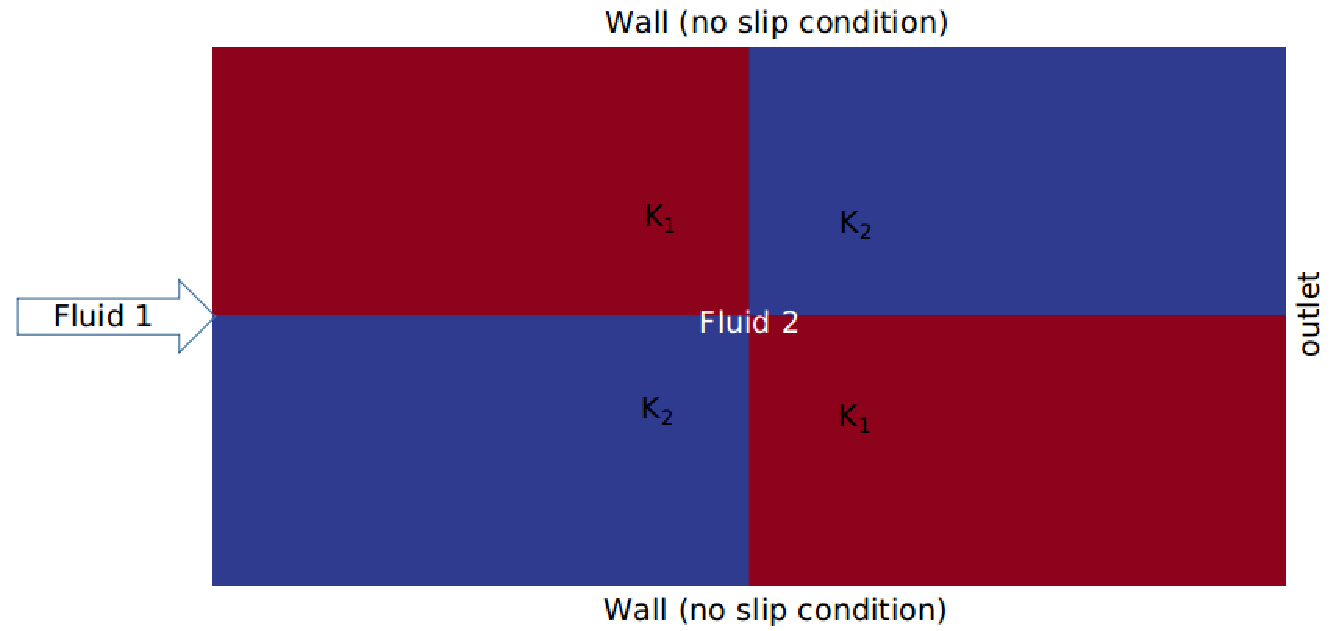
\includegraphics[width=.8\textwidth]{./Pics1/2b2_wi_fine/2b2_whole_in_fine_perm_1.pdf} 
}
\vspace{0.0cm}
\hbox{\hspace{3.5cm} (a) map of permeabilities ($\mathbf{K}$)
}
\vspace{0.25cm}
\hbox{\hspace{1.5cm}
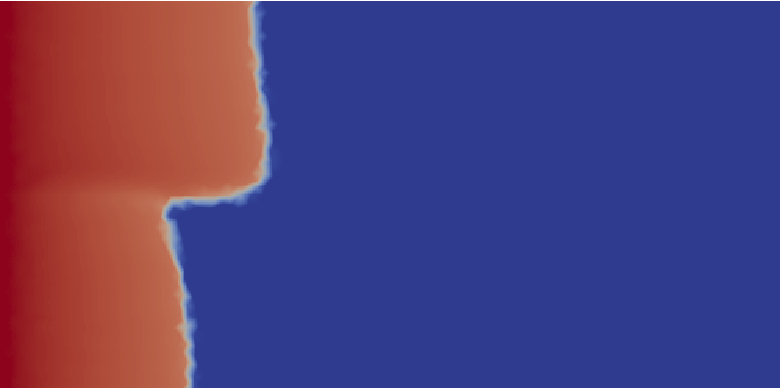
\includegraphics[width=.85\textwidth]{./Pics1/2b2_wi_fine/2b2_whole_in_fine_250_2.pdf}
}
\vspace{0.0cm}
\hbox{\hspace{4.5cm} (b) flow at t=250 
}
\vspace{0.25cm}
\hbox{\hspace{1.5cm}
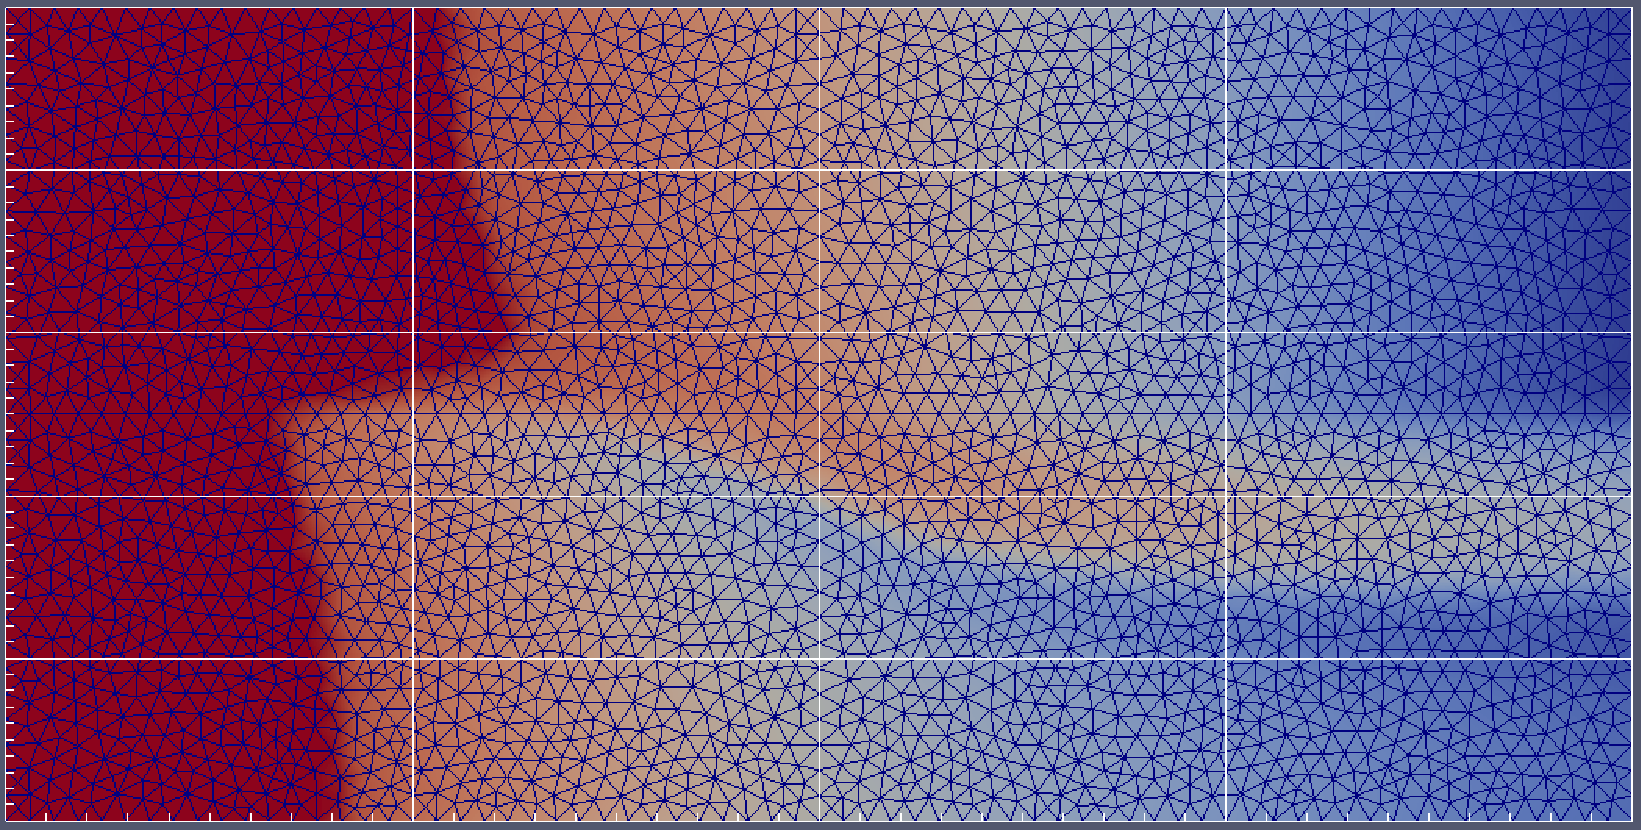
\includegraphics[width=.65\textwidth]{./Pics1/2b2_wi_fine/2b2_whole_in_fine_3000_2.pdf}
}
\vspace{0.0cm}
\hbox{\hspace{4.0cm} (c) flow at t=3000   
}}     
\caption{Model validation of fluid displacement in heterogeneous porous media ({\it VR}=1): (a) the domain is divided into four subdomains with prescribed synthetic permeability, $\mathbf{K}_{1}=1$ and $\mathbf{K}_{2}=2.5$; (b-c) snapshots of saturation (displacing fluid) field at t=$25$s and t=$300$ sec. The domain is discretised with $5960$ \PN[1]{2} elements. }
\label{fem_cv_represent_a}
\end{figure}
\clearpage



%%%%
%%%%  FIGURE
%%%%
\begin{landscape}
\begin{figure}[ht] 
\vbox{\vspace{-1cm}
\hbox{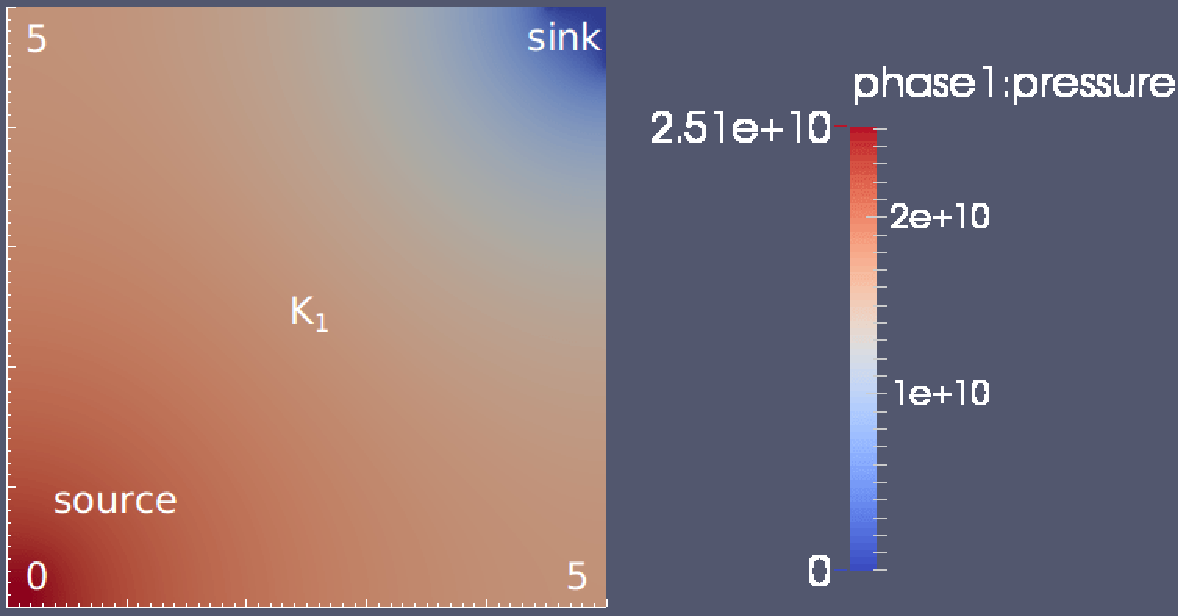
\includegraphics[width=.7\textwidth]{./Pics1/Saffman_homogeneous_MR3/saffman_homo_fixed_2.pdf}
      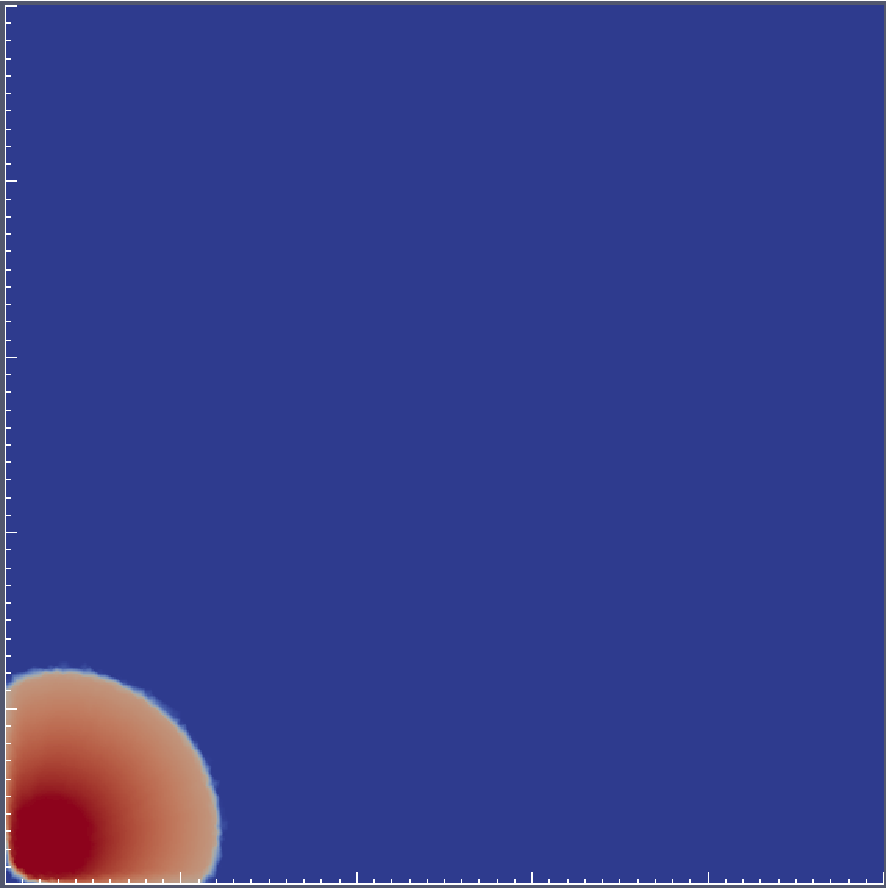
\includegraphics[width=.37\textwidth]{./Pics1/Saffman_homogeneous_MR3/saffman_homo_fixed_250.pdf}
      \includegraphics[width=.37\textwidth]{./Pics1/Saffman_homogeneous_MR3/saffman_homo_fixed_1000.pdf}}
\vspace{0.cm}
\hbox{\hspace{2.5cm} (a) pressure at t=0s \hspace{5.cm} (b) t=0.87s \hspace{2.75cm} (c) t=3.54s}
\vspace{0.5cm}
\hbox{
      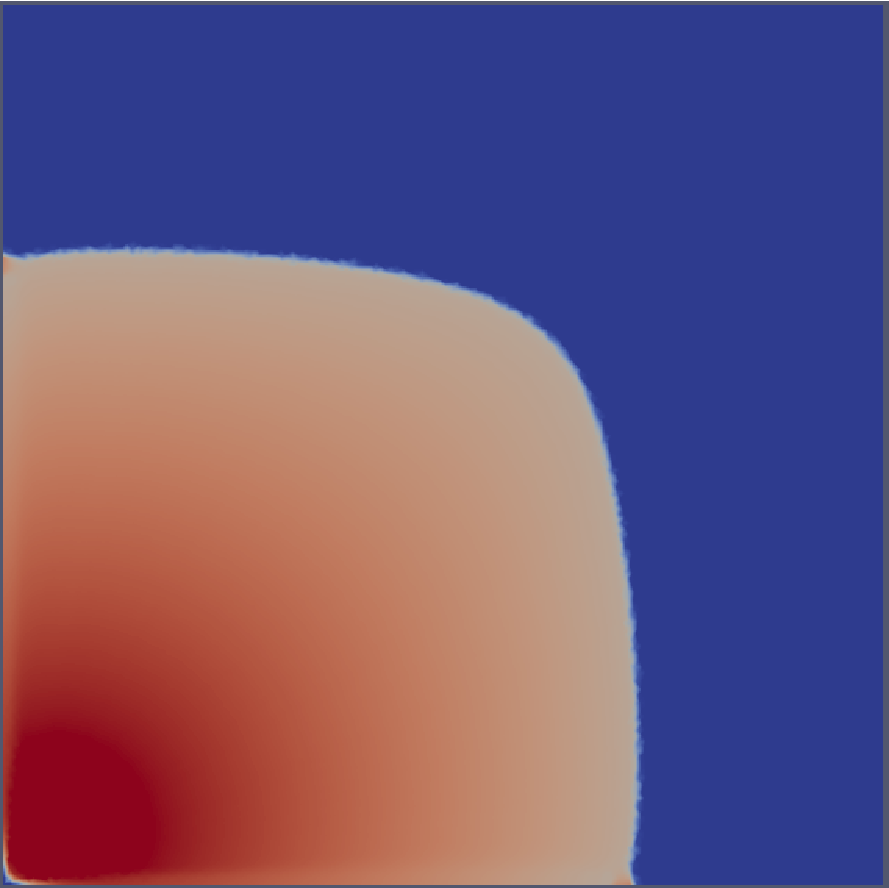
\includegraphics[width=.375\textwidth]{./Pics1/Saffman_homogeneous_MR3/saffman_homo_fixed_2500.pdf}
      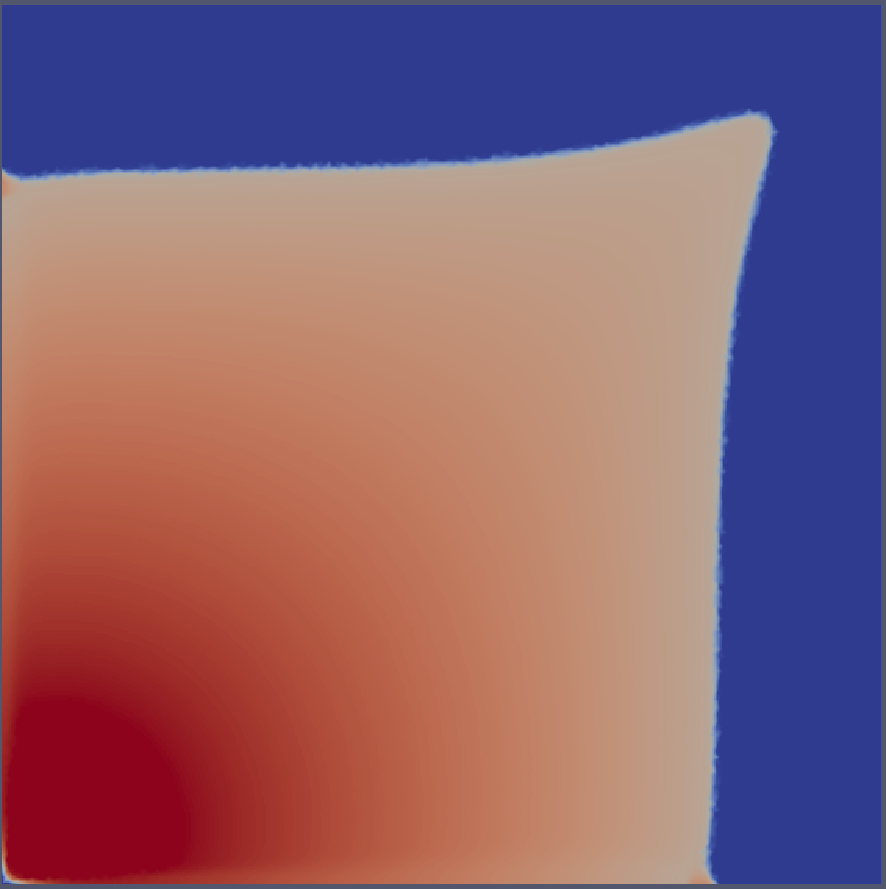
\includegraphics[width=.375\textwidth]{./Pics1/Saffman_homogeneous_MR3/saffman_homo_fixed_3500.pdf} 
      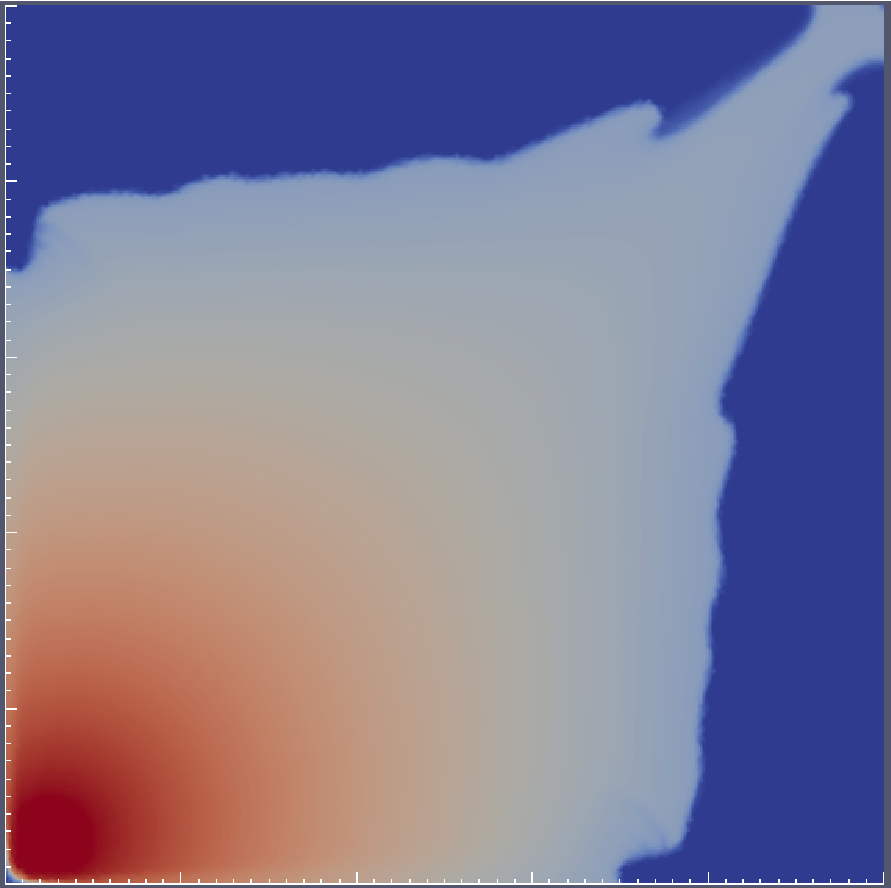
\includegraphics[width=.65\textwidth]{./Pics1/Saffman_homogeneous_MR3/saffman_homo_fixed_end.pdf}}
\vspace{0.cm}
\hbox{ \hspace{1.cm} (d) t=8.86s \hspace{3.0cm} (e) t=12.41s   \hspace{4.0cm} (f) t=17.95s}
\vspace{0.cm}
}   
\caption{Simulated flow in a Hele-Shaw cell ({\it VR}=3): (a) initial pressure profile $\left(\text{in g.cm}^{-1}\text{.s}^{-2}\right)$ with source and sink regions are explicitly shown along with dimensions (in cm); (b-f) snapshots of wetting phase saturation showing flow profile as the simulation evolves. The domain contains $47500$ \PN[1]{2} triangular elements.}
\label{fig:homoheleshaw_VN3}
\end{figure}
\end{landscape}
\clearpage



%%%%
%%%%  FIGURE
%%%%
\begin{landscape}
\begin{figure}[ht] 
\vbox{\vspace{-1cm}
\hbox{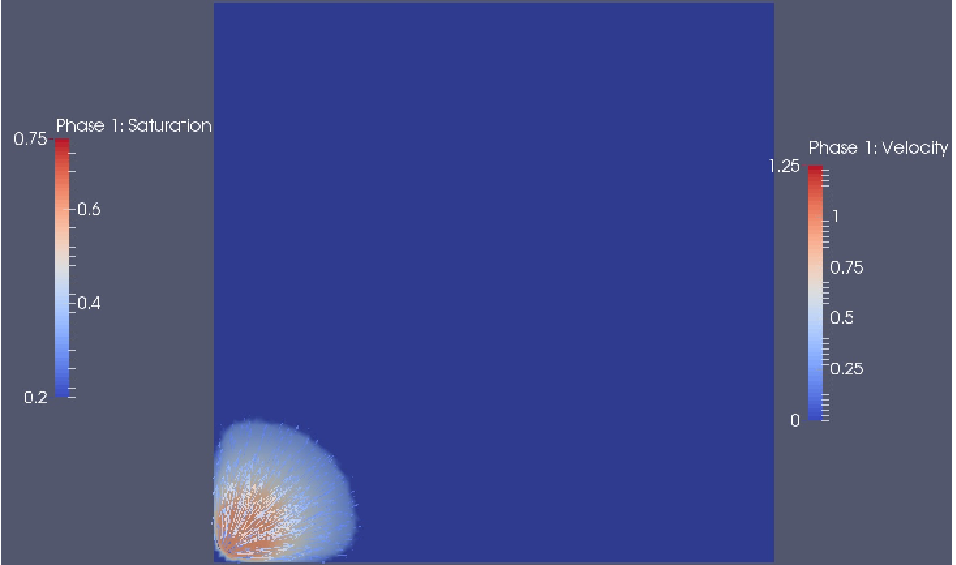
\includegraphics[width=.9\textwidth, height=0.5\textwidth]{./Pics1/Saffman_homogeneous_VR10/ST_Homog_VR10_D201c.pdf}
\hspace{0.5cm}      
      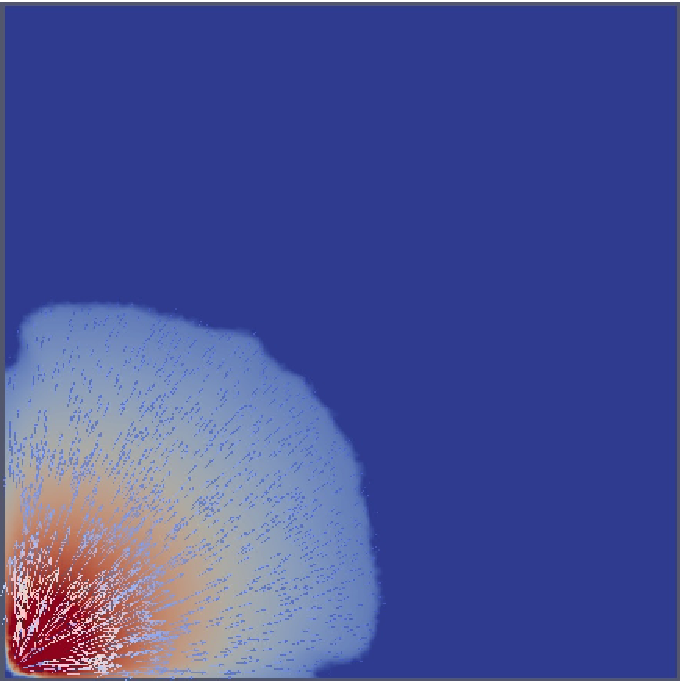
\includegraphics[width=.5\textwidth]{./Pics1/Saffman_homogeneous_VR10/ST_Homog_VR10_D1001c.pdf}}
\vspace{0.cm}
\hbox{\hspace{5.cm} (a) t=0.66s \hspace{8.cm} (b) t=3.43s }
\vspace{0.5cm}
\hbox{
      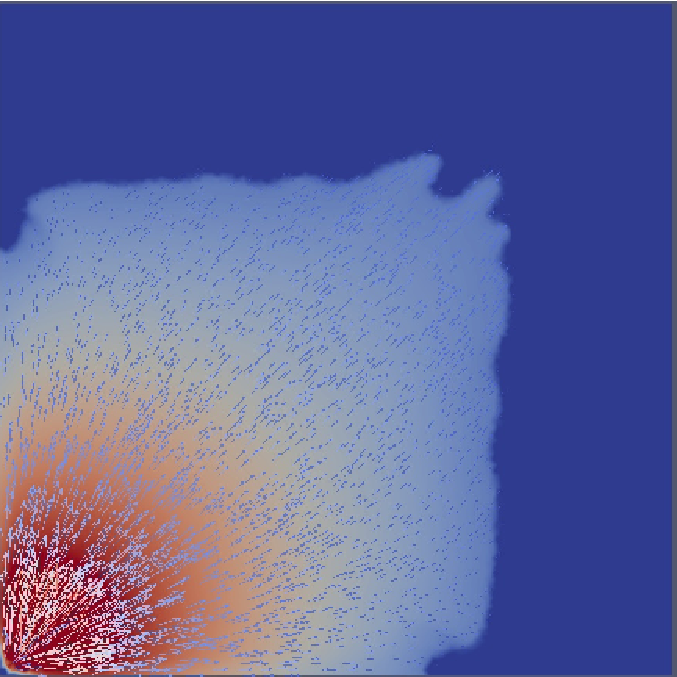
\includegraphics[width=.5\textwidth]{./Pics1/Saffman_homogeneous_VR10/ST_Homog_VR10_D2001c}
      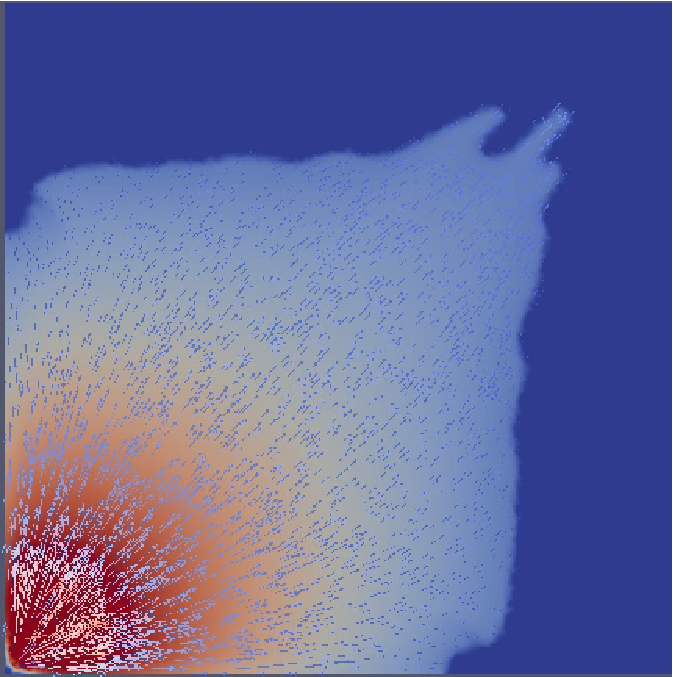
\includegraphics[width=.5\textwidth]{./Pics1/Saffman_homogeneous_VR10/ST_Homog_VR10_D2201c}
      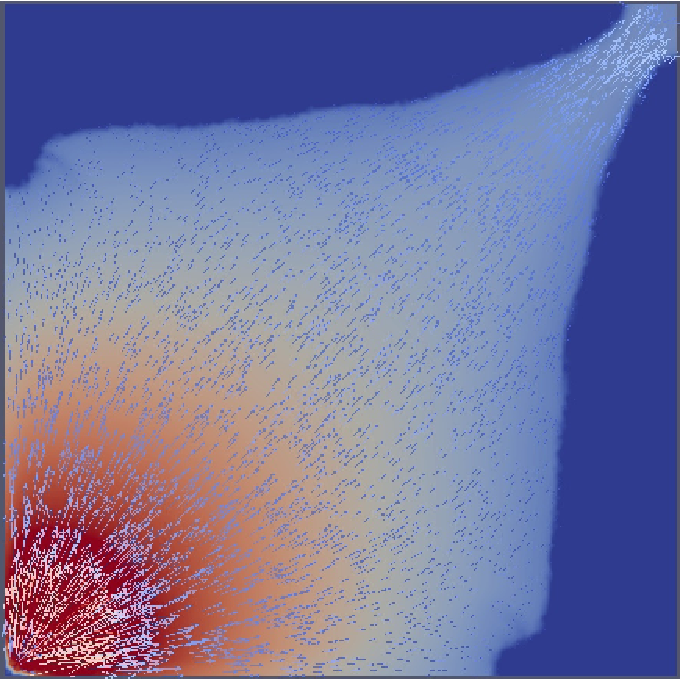
\includegraphics[width=.5\textwidth]{./Pics1/Saffman_homogeneous_VR10/ST_Homog_VR10_D3001c}}
\vspace{0.cm}
\hbox{ \hspace{2.cm} (c) t=6.92s \hspace{4.5cm} (d) t=7.61s \hspace{4.5cm} (e)t=10.00s}
\vspace{0.cm}
}   
\caption{Simulated flow in a Hele-Shaw cell ({\it VR}=10): snapshots of overlapped wetting phase saturation and velocity vectors showing flow profile as the simulation evolves. The domain contains $26313$ \PN[1]{2} triangular elements.}
\label{fig:homoheleshaw_VN10}
\end{figure}
\end{landscape}
\clearpage

%%%%
%%%%  FIGURE
%%%%
\begin{landscape}
\begin{figure}[ht] 
\vbox{\vspace{-1cm}
\hbox{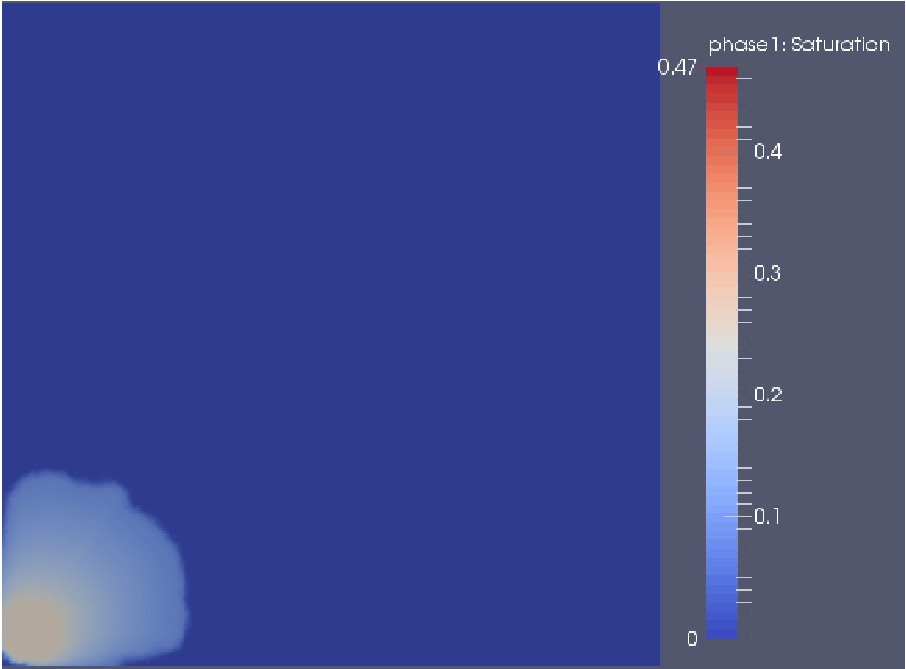
\includegraphics[width=.9\textwidth, height=0.5\textwidth]{./Pics1/Saffman_homogeneous_VR150/ST_Homog_VR150_D300b}
\hspace{0.5cm}      
      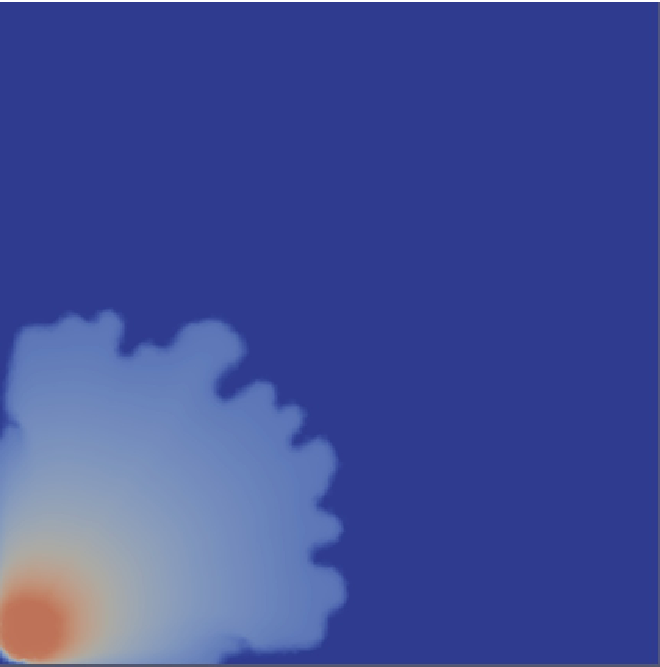
\includegraphics[width=.5\textwidth]{./Pics1/Saffman_homogeneous_VR150/ST_Homog_VR150_D1600b}}
\vspace{0.cm}
\hbox{\hspace{5.cm} (a) t=0.27s \hspace{8.cm} (b) t=0.94s }
\vspace{0.5cm}
\hbox{
      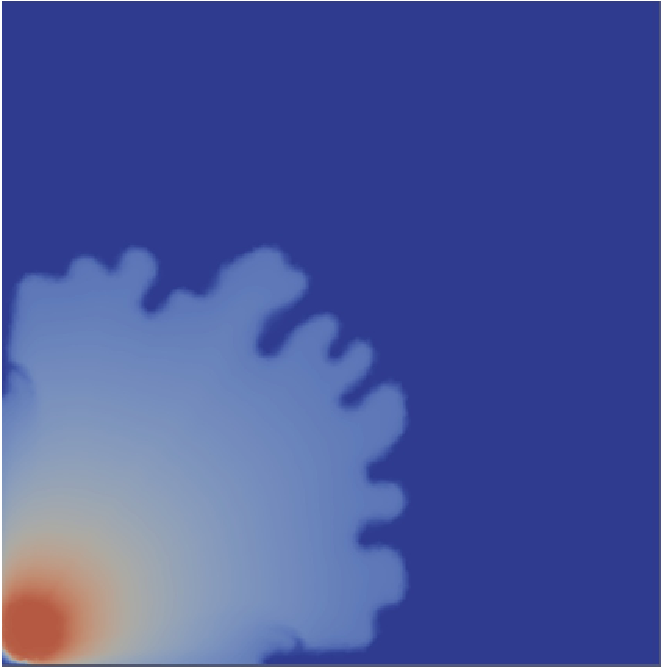
\includegraphics[width=.5\textwidth]{./Pics1/Saffman_homogeneous_VR150/ST_Homog_VR150_D2700b}
      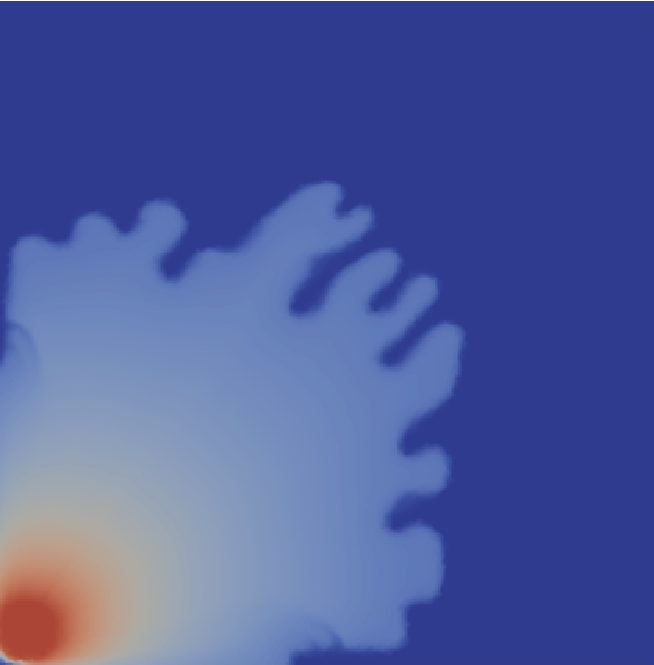
\includegraphics[width=.5\textwidth]{./Pics1/Saffman_homogeneous_VR150/ST_Homog_VR150_D4000b}
      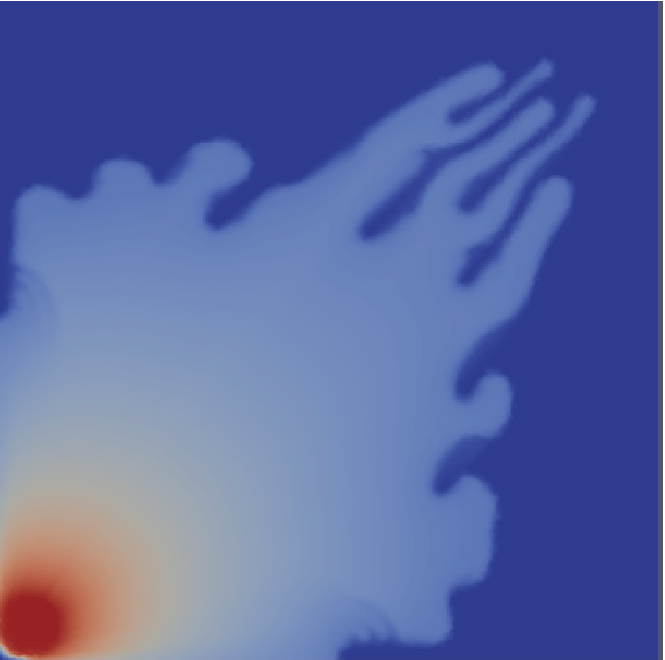
\includegraphics[width=.5\textwidth]{./Pics1/Saffman_homogeneous_VR150/ST_Homog_VR150_D7000b}}
\vspace{0.cm}
\hbox{ \hspace{2.cm} (c) t=1.32s \hspace{4.5cm} (d) t=1.70s \hspace{4.5cm} (e)t=2.31s}
\vspace{0.cm}
}   
\caption{Simulated flow in a Hele-Shaw cell ({\it VR}=150): snapshots of wetting phase saturation showing flow profile as the simulation evolves. The domain contains $26313$ \PN[1]{2} triangular elements.}
\label{fig:homoheleshaw_VN10}
\end{figure}
\end{landscape}
\clearpage


%%%%
%%%%  FIGURE
%%%%
\begin{landscape}
\begin{figure}[ht] 
\hbox{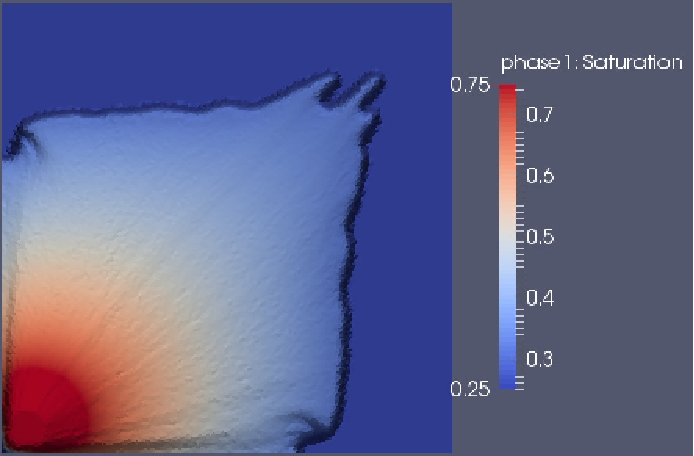
\includegraphics[width=.5\textwidth]{./Pics1/Saffman_homogeneous_VR10/ST_Homog_VR10_D2201_bbd}
       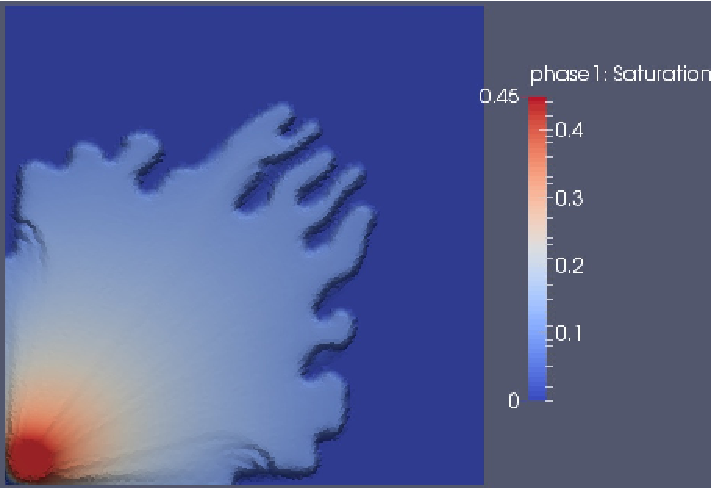
\includegraphics[width=.49\textwidth]{./Pics1/Saffman_homogeneous_VR150/ST_Homog_VR150_D5003_k2b}}
\caption{Simulated flow in Hele-Shaw cells performed with viscosity ratios of 10 (left, t=7.61s) and 150 (t=1.94s). Width of largest fingers are approximetely 0.70 and 0.90cm, which are in good agreement with values obtained from \citet{guan_2003}'s analytic solution. Domains of both simulations contain $26313$ \PN[1]{2} triangular elements.\red{(More pics to be added!!)}}
\label{fig:homoheleshaw_VN10_VN150}
\end{figure}
\end{landscape}



\begin{comment}

%%%%
%%%%  FIGURE
%%%%
\begin{landscape}
\begin{figure}[ht] 
\vbox{\vspace{-1cm}
\hbox{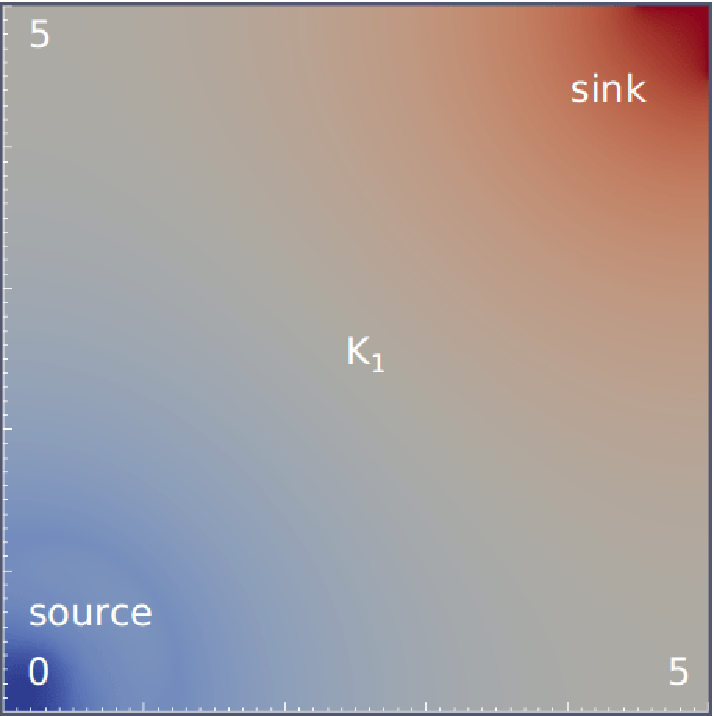
\includegraphics[width=.5\textwidth]{./Pics1/Saffman_homogeneous/saffman_homo_fixed_1.pdf}
      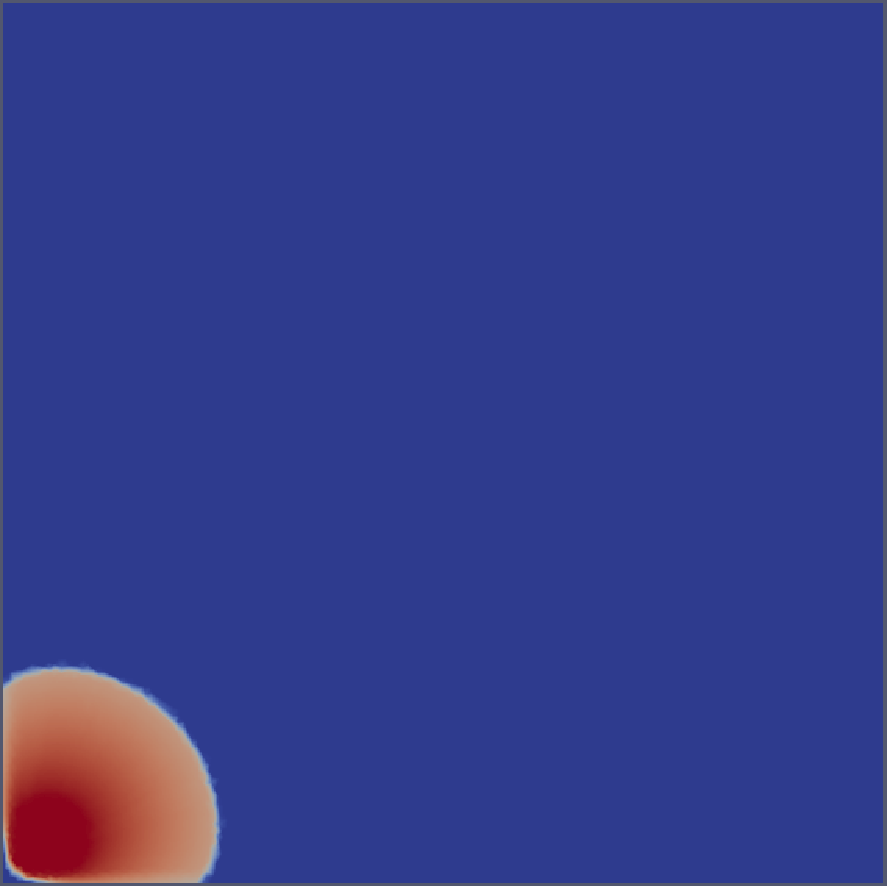
\includegraphics[width=.5\textwidth]{./Pics1/Saffman_homogeneous/saffman_homo_fixed_250_1.pdf}
      \includegraphics[width=.5\textwidth]{./Pics1/Saffman_homogeneous/saffman_homo_fixed_1000.pdf}}
\vspace{0.cm}
\hbox{\hspace{1.0cm} (a) pressure at t=0 \hspace{3.cm} (b) t=250\red{(???)} \hspace{3.0cm} (c) t=1000\red{(???)}}
\vspace{0.5cm}
\hbox{
      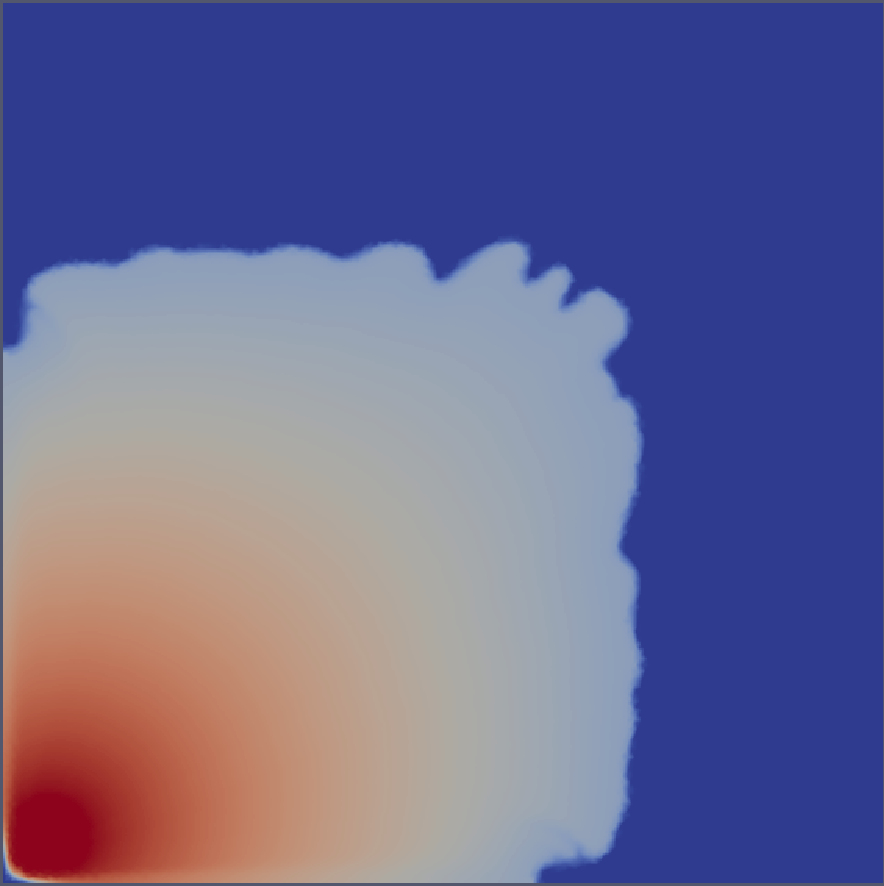
\includegraphics[width=.5\textwidth]{./Pics1/Saffman_homogeneous/saffman_homo_fixed_6000.pdf}
      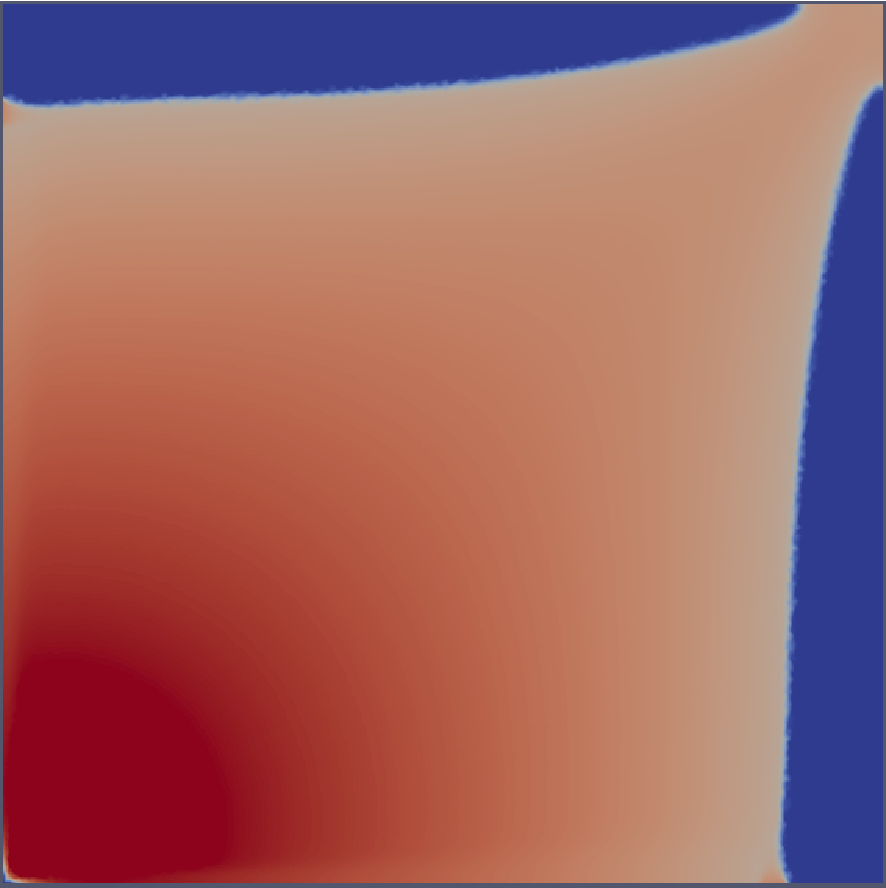
\includegraphics[width=.5\textwidth]{./Pics1/Saffman_homogeneous/saffman_homo_fixed_end_1.pdf}}
\vspace{0.cm}
\hbox{ \hspace{2.cm} (d) t=6000\red{(???)} \hspace{3.cm} (e) t=XXX\red{(???)}}
\vspace{0.cm}
}   
\caption{Simulated flow in a Hele-Shaw cell ({\it VR}=10): (a) pressure profile $\left(\text{in g.cm}^{-1}\text{.s}^{-2}\right)$ with source and sink regions explicitly shown along with dimensions (in cm); (b-e) snapshots of wetting phase saturation showing flow profile as the simulation evolves. The domain contains $47000$ \PN[1]{2} triangular elements. The pressure and saturation range of values are the same like the  case in fig.\ref{fig:homoheleshaw_VN3}.}
\label{fig:homoheleshaw_VN10}
\end{figure}
\end{landscape}
\clearpage
\end{comment}


%%%
%%% FIGURE XXXXXX
%%%
\begin{landscape}
  \begin{figure}[ht]
  \vbox{\vspace{-1cm}
      \hbox{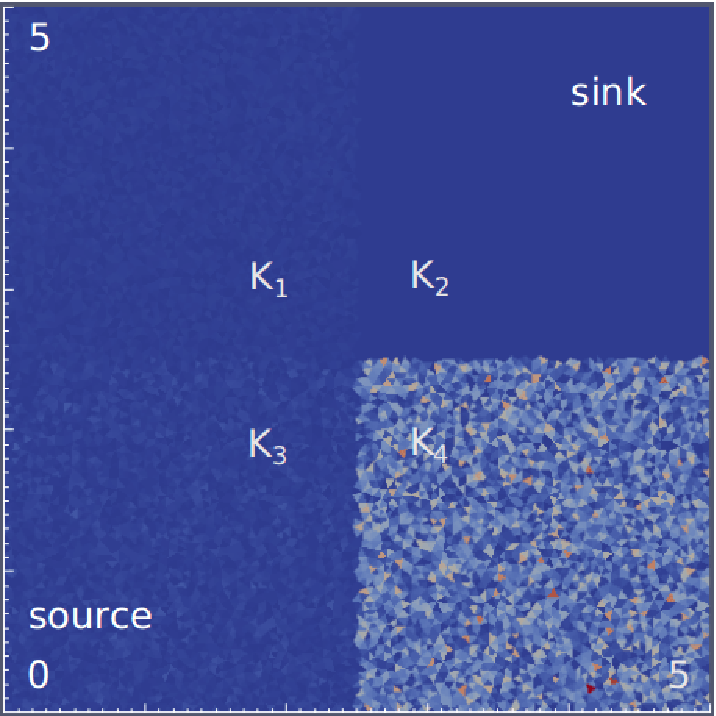
\includegraphics[width=.5\textwidth]{./Pics1/Saffman_heterogeneous/saffman_heter_fixed_1.pdf}
            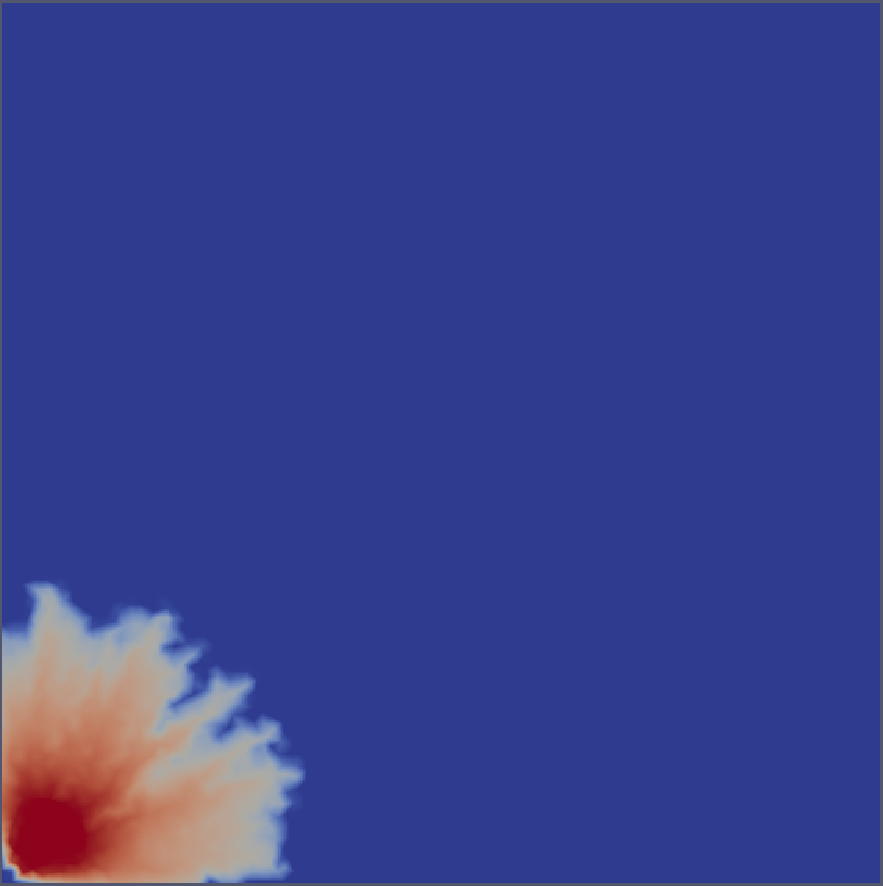
\includegraphics[width=.5\textwidth]{./Pics1/Saffman_heterogeneous/saffman_heter_fixed_500.pdf} 
            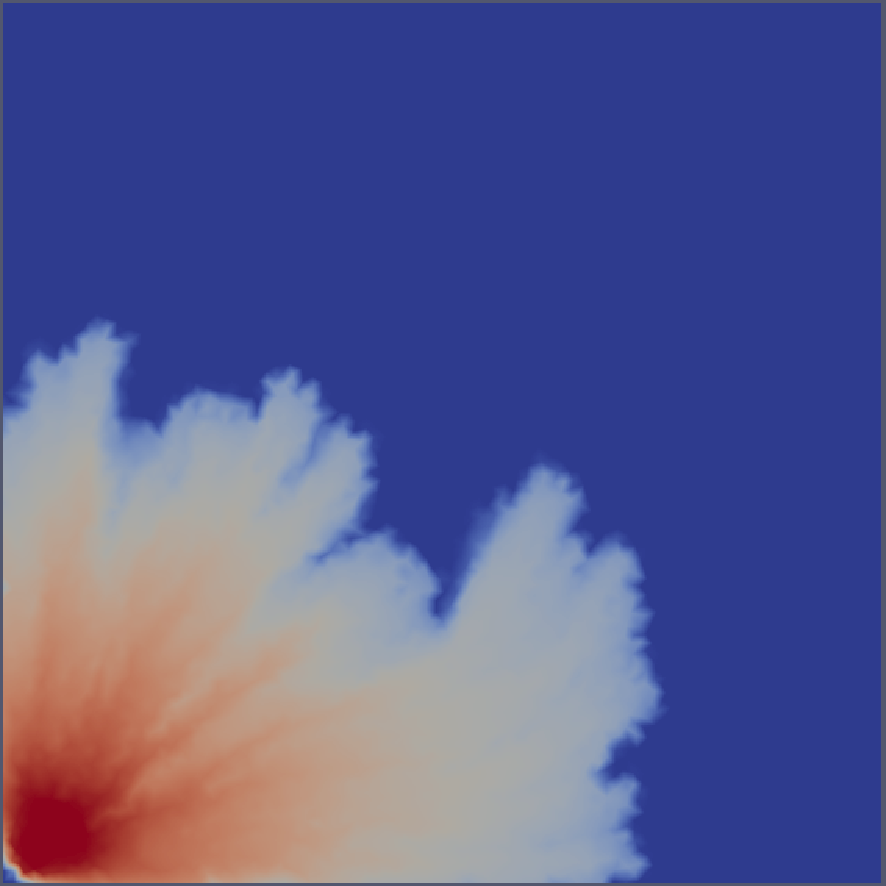
\includegraphics[width=.5\textwidth]{./Pics1/Saffman_heterogeneous/saffman_heter_fixed_2000.pdf} }
      \hbox{\hspace{1.0cm} (a) permeability map \hspace{3.cm} (b) t=0.75s \hspace{4.0cm} (c) t=8s}
      \vspace{0.5cm}
      \hbox{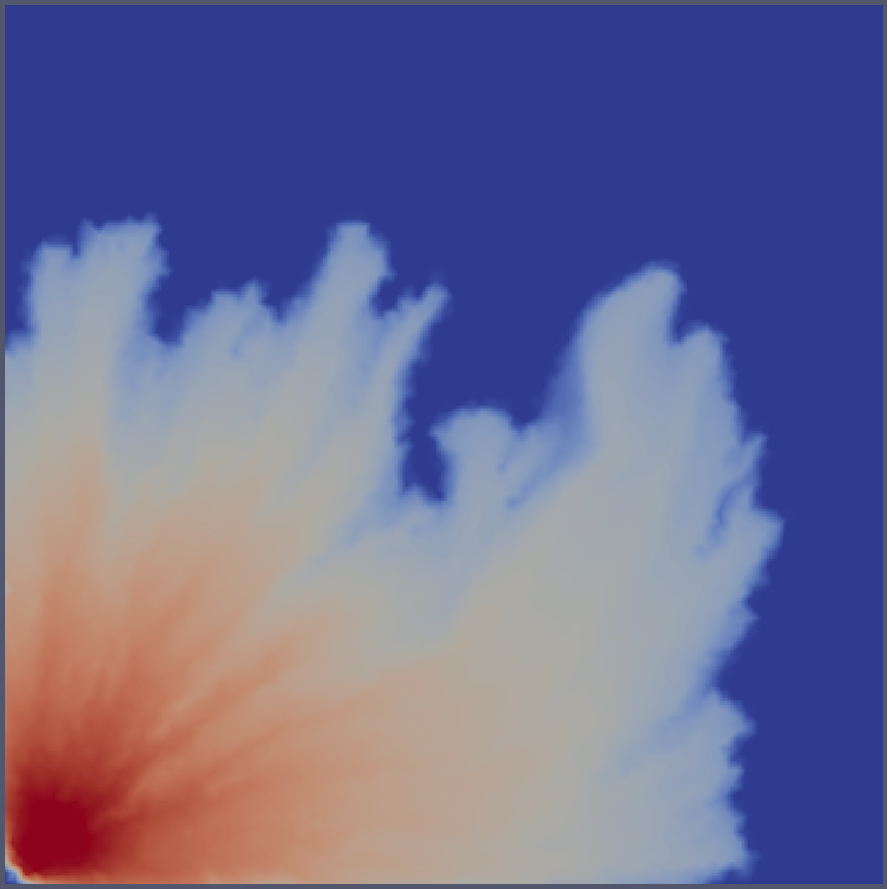
\includegraphics[width=.5\textwidth]{./Pics1/Saffman_heterogeneous/saffman_heter_fixed_3000.pdf}
            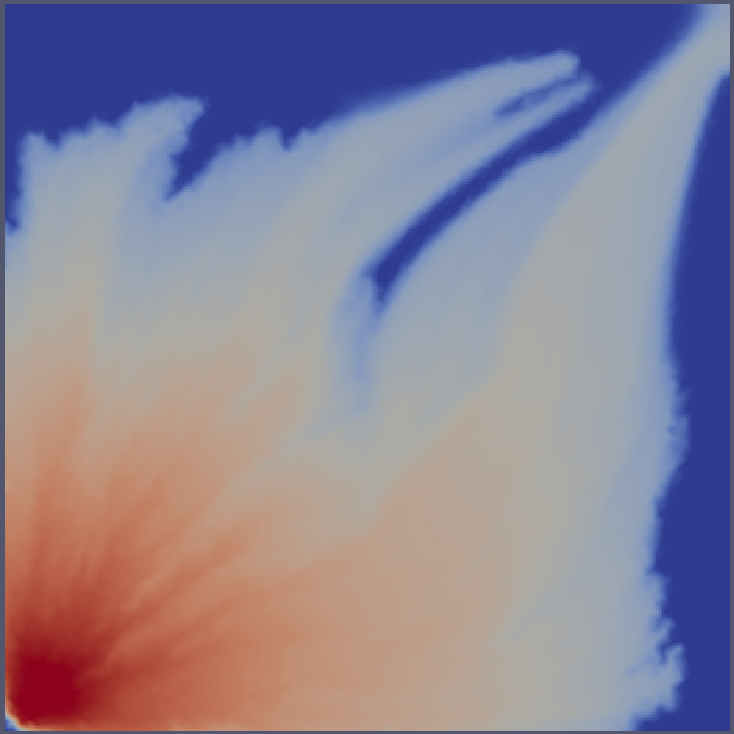
\includegraphics[width=.5\textwidth]{./Pics1/Saffman_heterogeneous/saffman_heter_fixed_6000.pdf}
            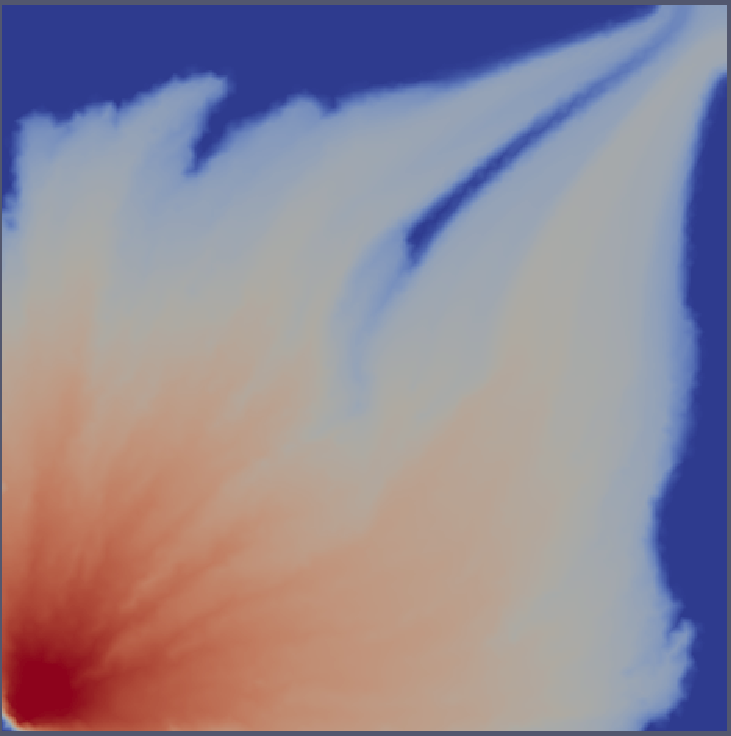
\includegraphics[width=.5\textwidth]{./Pics1/Saffman_heterogeneous/saffman_heter_fixed_24000.pdf} }
      \hbox{\hspace{2.5cm} (d) t=18s \hspace{5.cm} (e) t= \hspace{3.0cm} (f) t=24000 }}
\caption{Simulated flow in a modified Hele-Shaw cell with {\it VR}=10: (a) permeability distribution $\left(\text{10}^{-10}\le\mathbf{K}_{1}\le\text{5}\times\text{10}^{-10}\right.$, {\bf K}$_{2}$=10$^{-10}$, 10$^{-11}\le\mathbf{K}_{3}\le$ 5$\times$10$^{-10}$ and 10$^{-12}\le\mathbf{K}_{4}\le$ 5$\times$10$\left.^{-10}\text{ cm}^{2}\right)$; (b-f) snapshots of saturation profile during \red{XX} seconds of simulation. The domain contains \red{XX} \PN[1]{2} element-pairs.}
\label{fig:HeleShawHeter_VR10}
\end{figure}
\end{landscape}
\clearpage



%%%%
%%%%  FIGURE
%%%%
\begin{landscape}
\begin{figure}[ht] 
\vbox{
\hbox{\hspace{4.0cm}
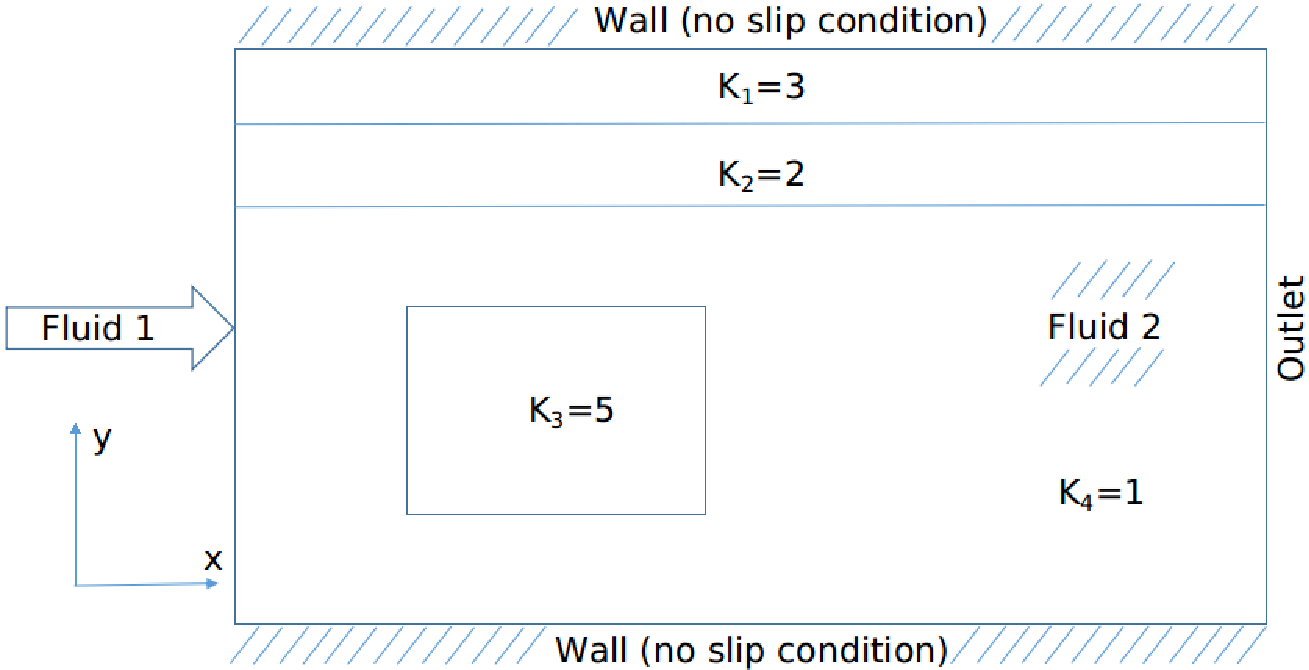
\includegraphics[width=.75\textwidth]{./Pics/map_of_boundaries.pdf} 
}
\vspace{0.0cm}
\hbox{\hspace{6.5cm} (a) map of permeabilties K   
}
\vspace{0.25cm}
\hbox{\hspace{4.0cm}
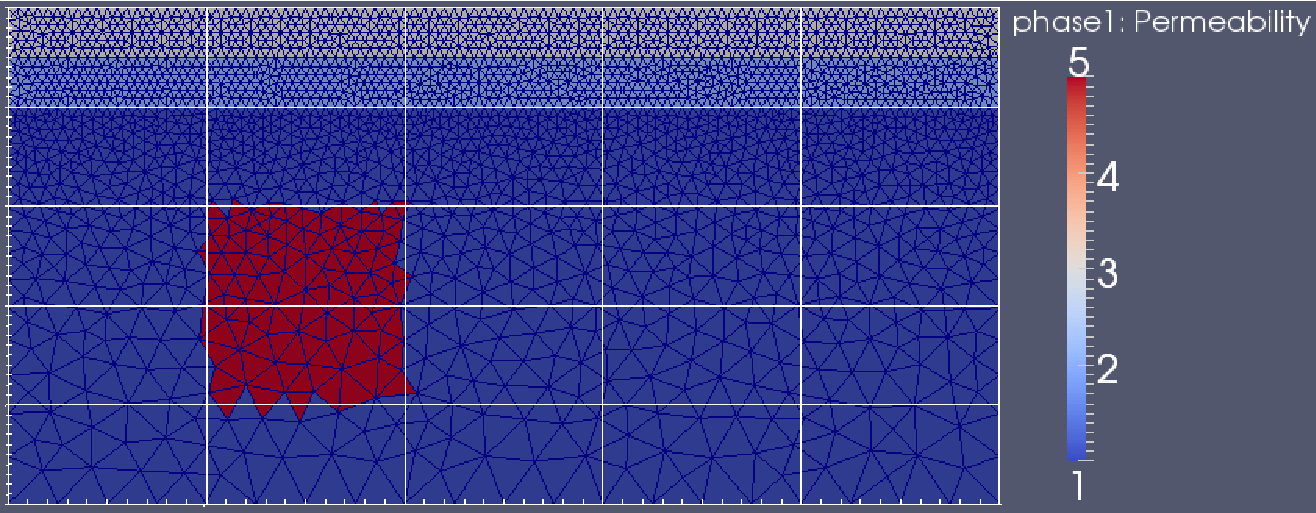
\includegraphics[width=.9\textwidth]{./Pics/map_of_boundaries_1.pdf}
}
\vspace{0.0cm}
\hbox{\hspace{9cm} (b)      
}
}     
\caption{Figure (a) describes the initial and boundary conditions as these are applied in this set of simulations. Below (b) there is a comparison between the unstructured and fixed mesh and the unstructured and adaptive mesh. During the implementation of fixed mesh initially there $4606$ elements while for the adaptive mesh there are $606$ while the majority of them is on the interface between between the two fluids. }
\label{fig:testcase_heter_domain}
\end{figure}
\end{landscape}
\clearpage



%%%%
%%%%  FIGURE
%%%%
\begin{landscape}
\begin{figure}[ht] 
\vbox{
\hbox{\hspace{3.5cm}
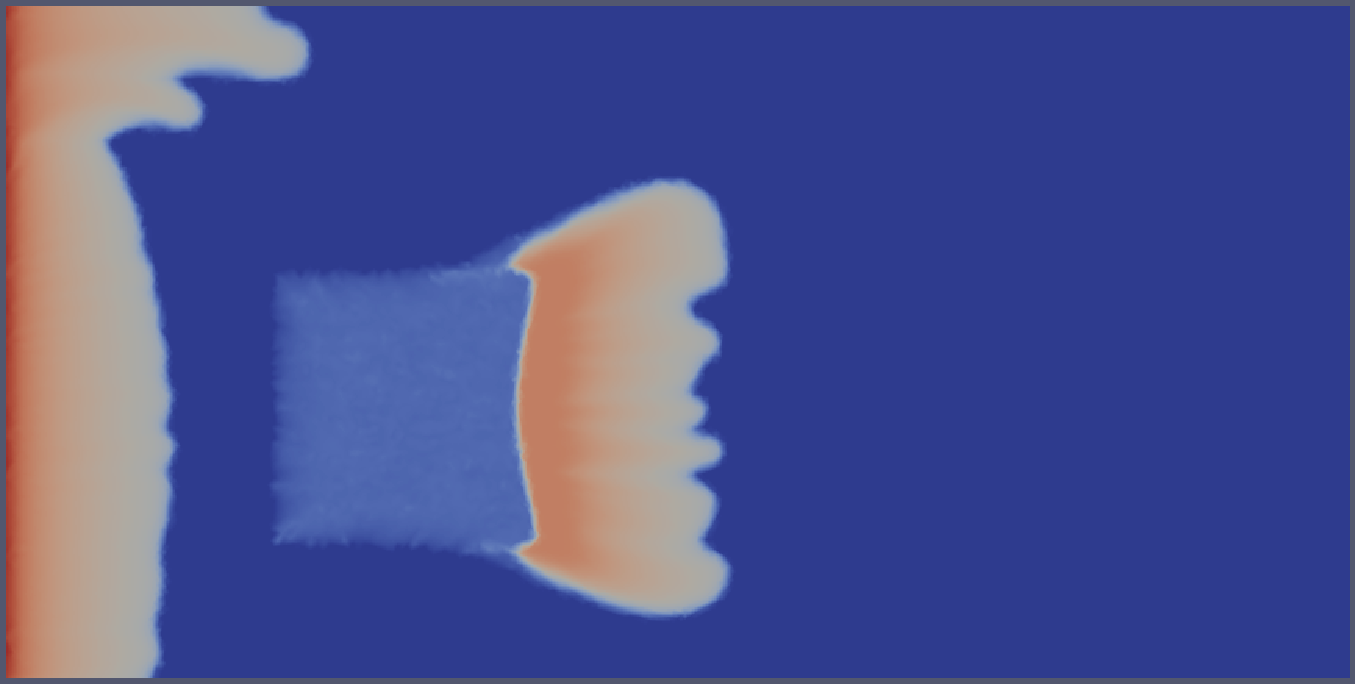
\includegraphics[width=.65\textwidth]{./Pics1/mr10_5regions_fixed/5regions_fixed_250.pdf} 
}
\vspace{0.0cm}
\hbox{\hspace{6.5cm} (a) flow at t=250 (fixed mesh)  
}
\vspace{0.25cm}
\hbox{\hspace{3.5cm}
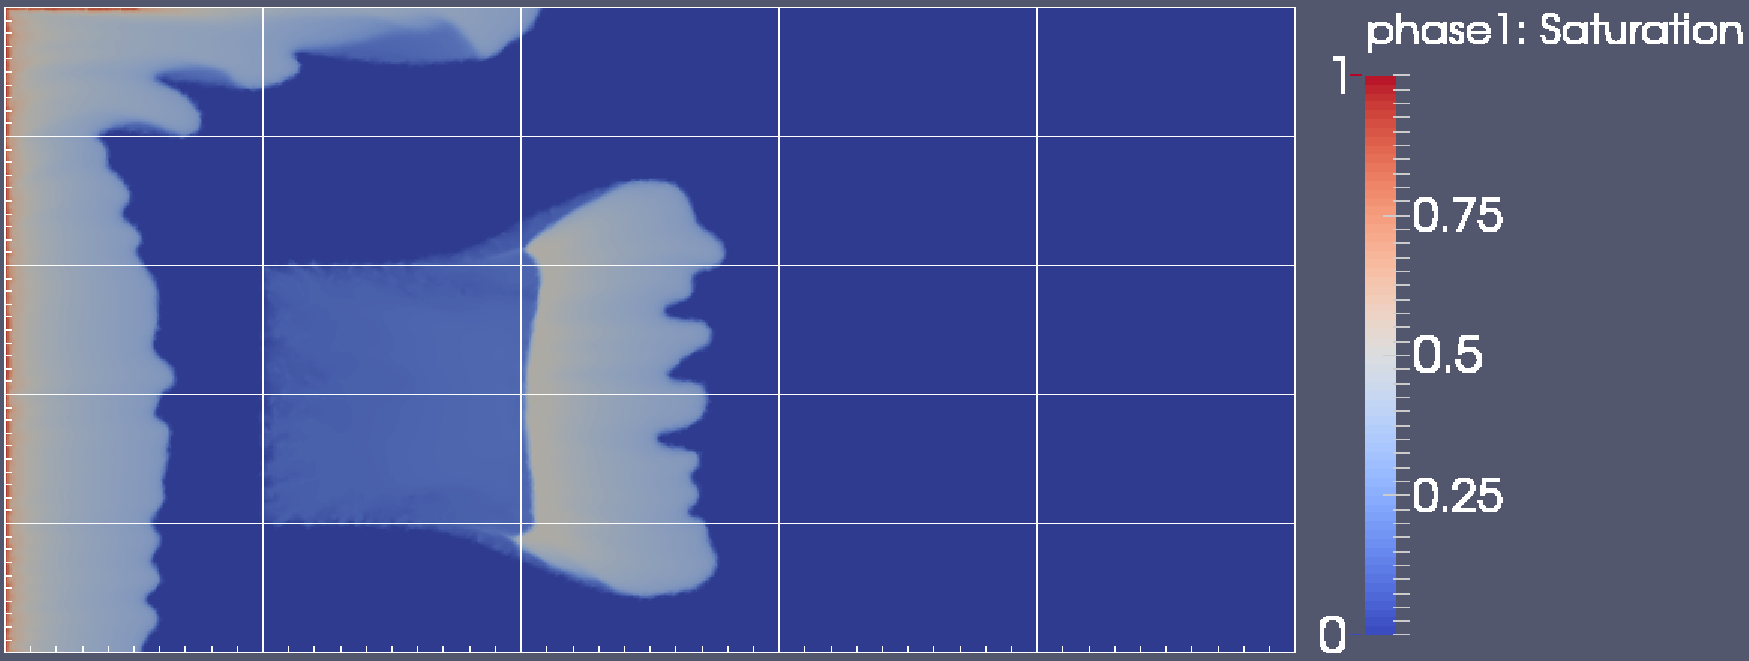
\includegraphics[width=.9\textwidth]{./Pics1/mr10_5regions_adapt/5regions_adapt_250_1.pdf}
}
\vspace{0.0cm}
\hbox{\hspace{6.5cm} (b) flow at t=250 (adaptive mesh)    
}
}     
\caption{For $t=0.125$s, $2$ test-cases under the VR=$10$ and under fixed (top) and adaptive(bottom) mesh are compared. There is a significant difference on the main front (left hand side of the domain) and the number of finger that appear.}
\label{fig:2testcase_a}
\end{figure}
\end{landscape}
\clearpage


%%%%
%%%%  FIGURE
%%%%
\begin{landscape}
\begin{figure}[ht] 
\vbox{
\hbox{\hspace{3.5cm}
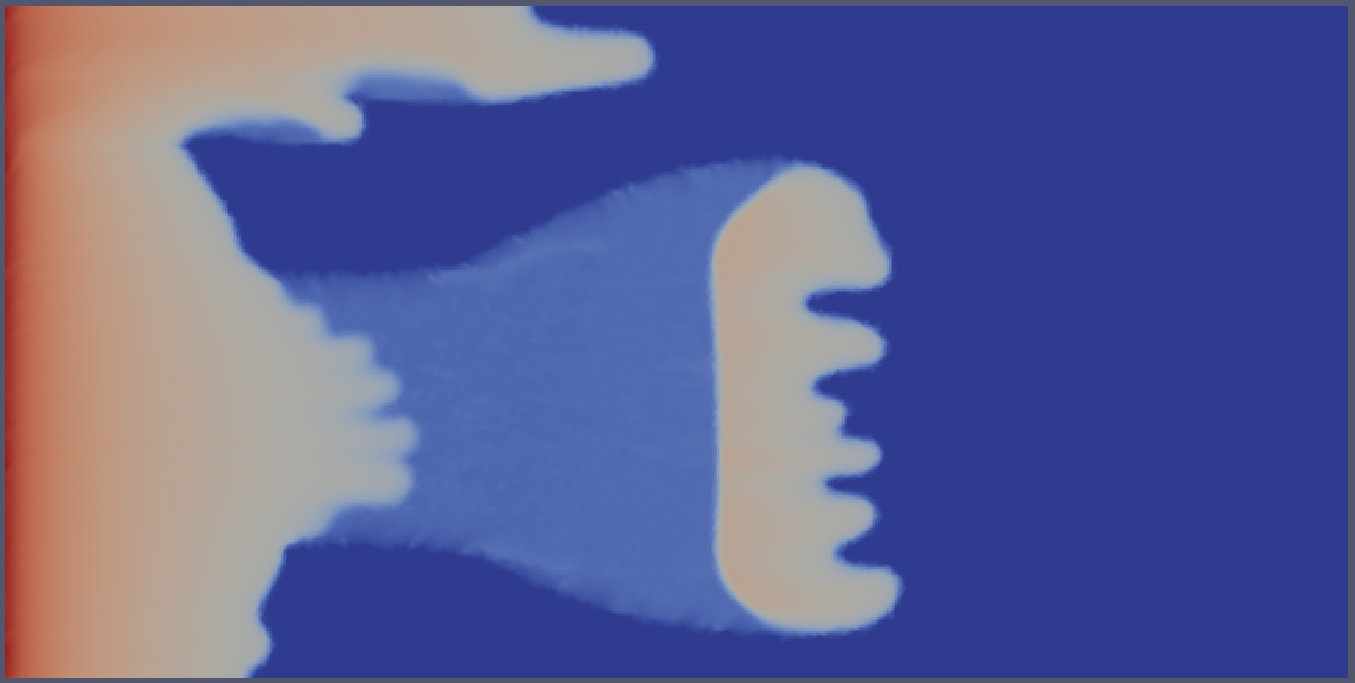
\includegraphics[width=.65\textwidth]{./Pics1/mr10_5regions_fixed/5regions_fixed_500.pdf} 
}
\vspace{0.0cm}
\hbox{\hspace{6.5cm} (a) flow at t=500 (fixed mesh)   
}
\vspace{0.25cm}
\hbox{\hspace{3.5cm}
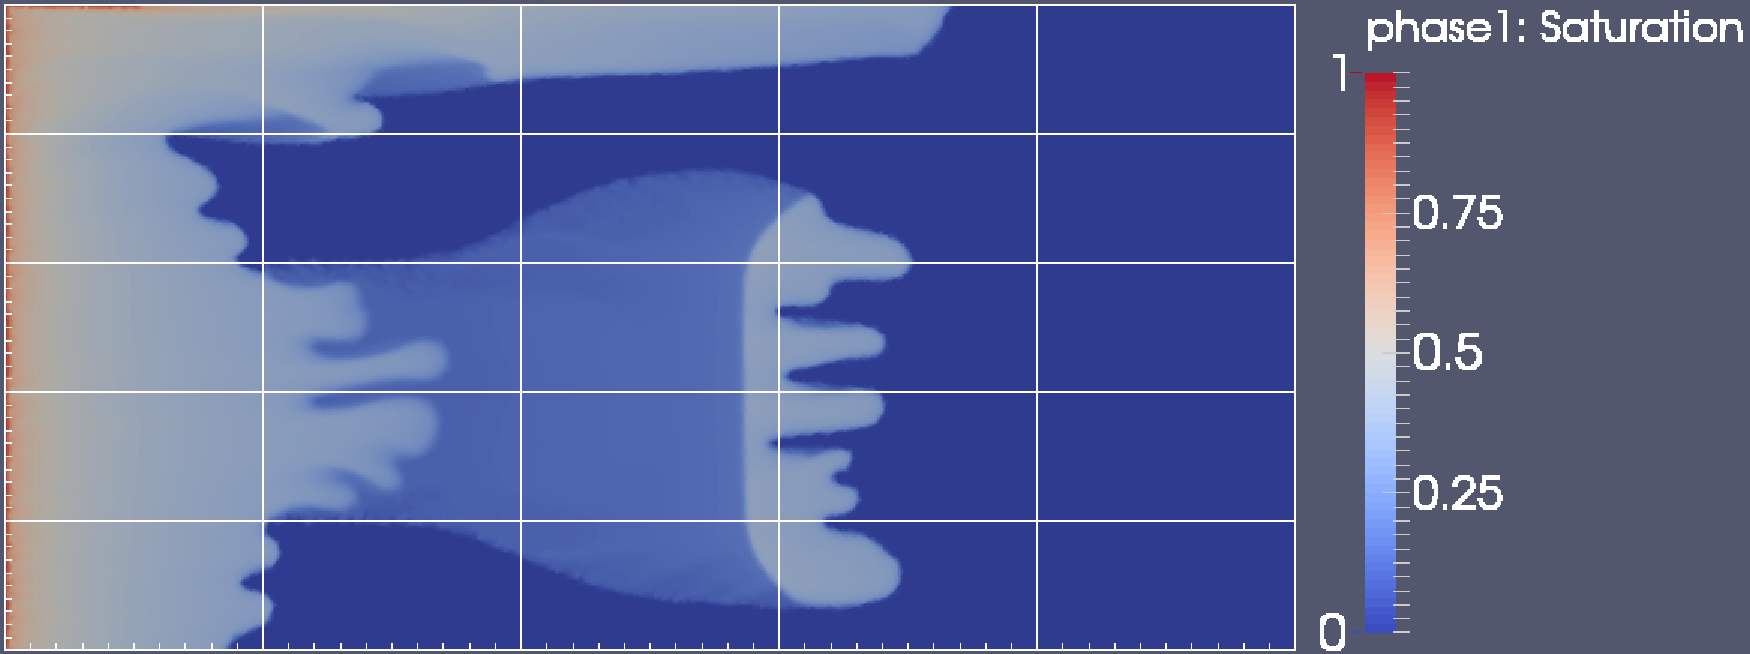
\includegraphics[width=.9\textwidth]{./Pics1/mr10_5regions_adapt/5regions_adapt_500_1.pdf}
}
\vspace{0.0cm}
\hbox{\hspace{6.5cm} (b) flow at t=500 (adaptive mesh)     
}
}     
\caption{At $t=0.25$s ($t=500$, timestemp) cross flow is taking place at the upper part of the formation. The fingers start to becoming more proufound as can been seen at the bottom.}
\label{fig:2testcase_b}
\end{figure}
\end{landscape}
\clearpage



%%%%
%%%%  FIGURE
%%%%
\begin{landscape}
\begin{figure}[ht] 
\vbox{
\hbox{\hspace{3.5cm}
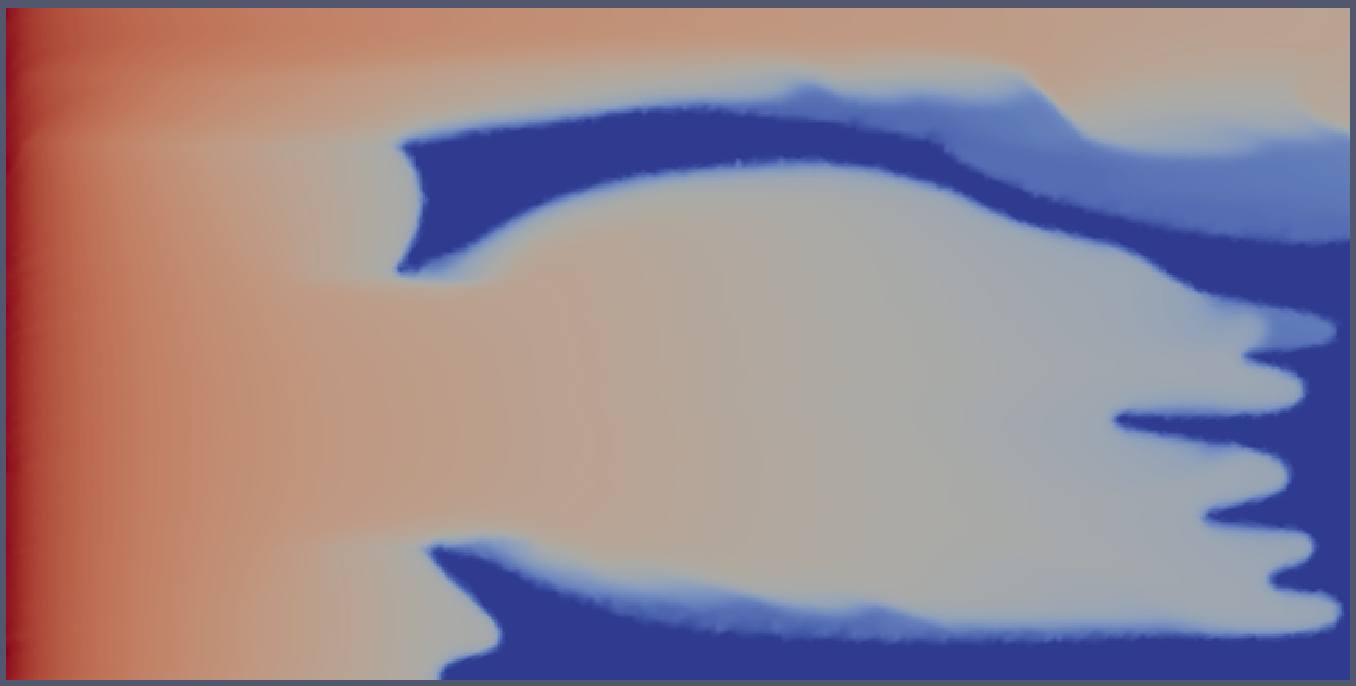
\includegraphics[width=.65\textwidth]{./Pics1/mr10_5regions_fixed/5regions_fixed_1500.pdf} 
}
\vspace{0.0cm}
\hbox{\hspace{6.5cm} (a) flow at t=1500 (fixed mesh)   
}
\vspace{0.25cm}
\hbox{\hspace{3.5cm}
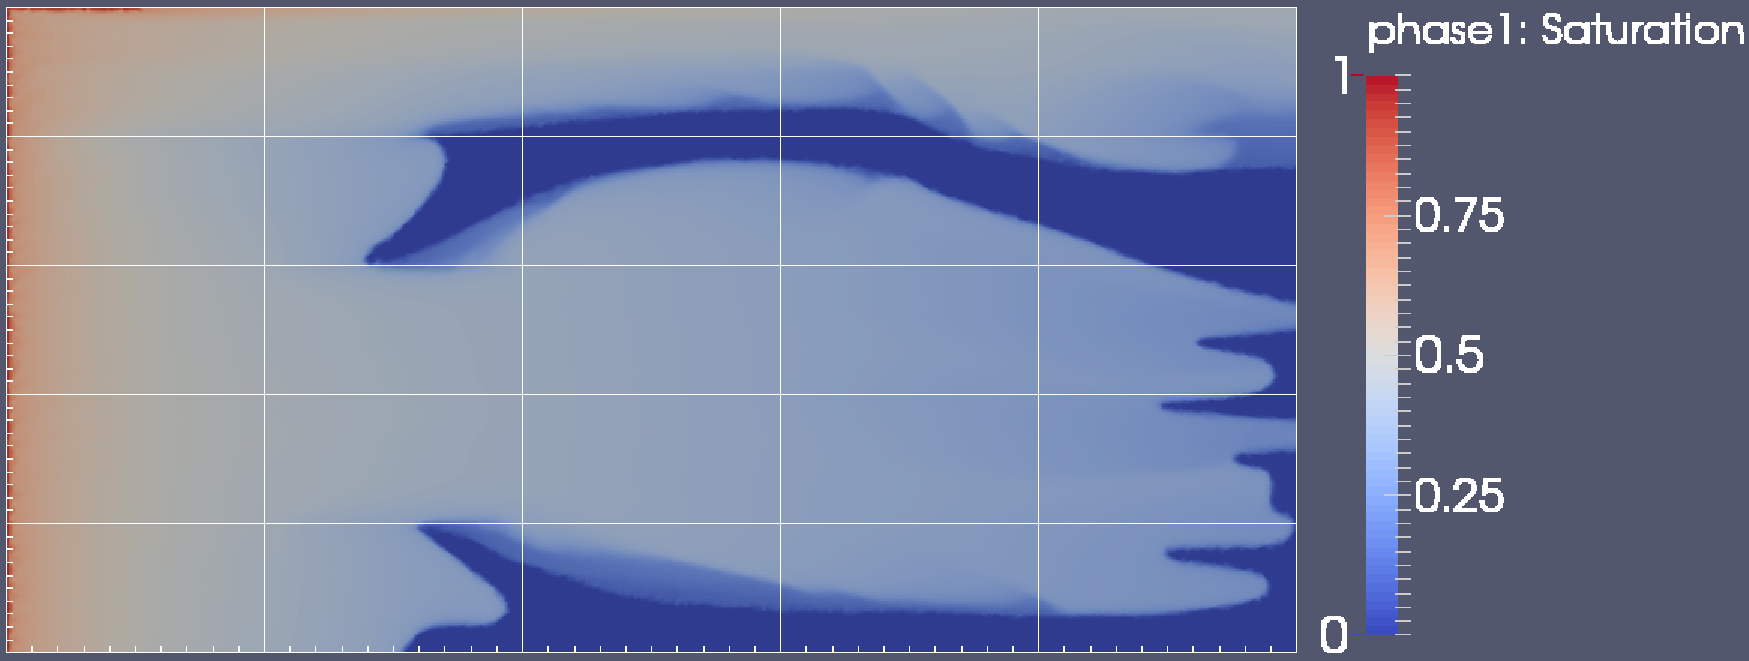
\includegraphics[width=.9\textwidth]{./Pics1/mr10_5regions_adapt/5regions_adapt_1500_1.pdf}
}
\vspace{0.0cm}
\hbox{\hspace{6.5cm} (b) flow at t=1500 (adaptive mesh)     
}
}     
\caption{At $t=0.75 sec$ ($t=1500$, timestemp) the initial cross flow is now fully developed and has travel all the way towards the outlet (right-hand side). and the finger below start forming a front that is also travelling towards the left-hand side.}
\label{fig:2testcase_c}
\end{figure}
\end{landscape}
\clearpage



%%%%
%%%%  FIGURE
%%%%
\begin{landscape}
\begin{figure}[ht] 
\vbox{
\hbox{\hspace{3.5cm}
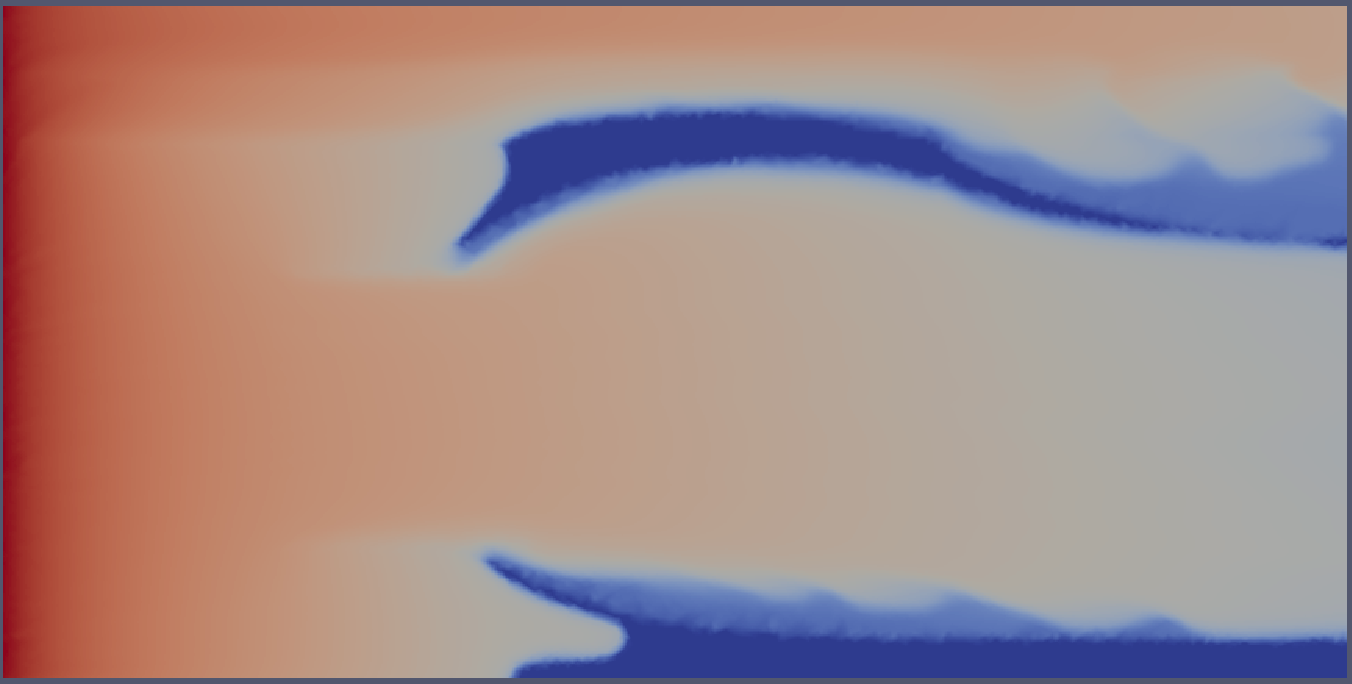
\includegraphics[width=.65\textwidth]{./Pics1/mr10_5regions_fixed/5regions_fixed_2000.pdf} 
}
\vspace{0.0cm}
\hbox{\hspace{6.5cm} (a) flow at t=end (fixed mesh)   
}
\vspace{0.25cm}
\hbox{\hspace{3.5cm}
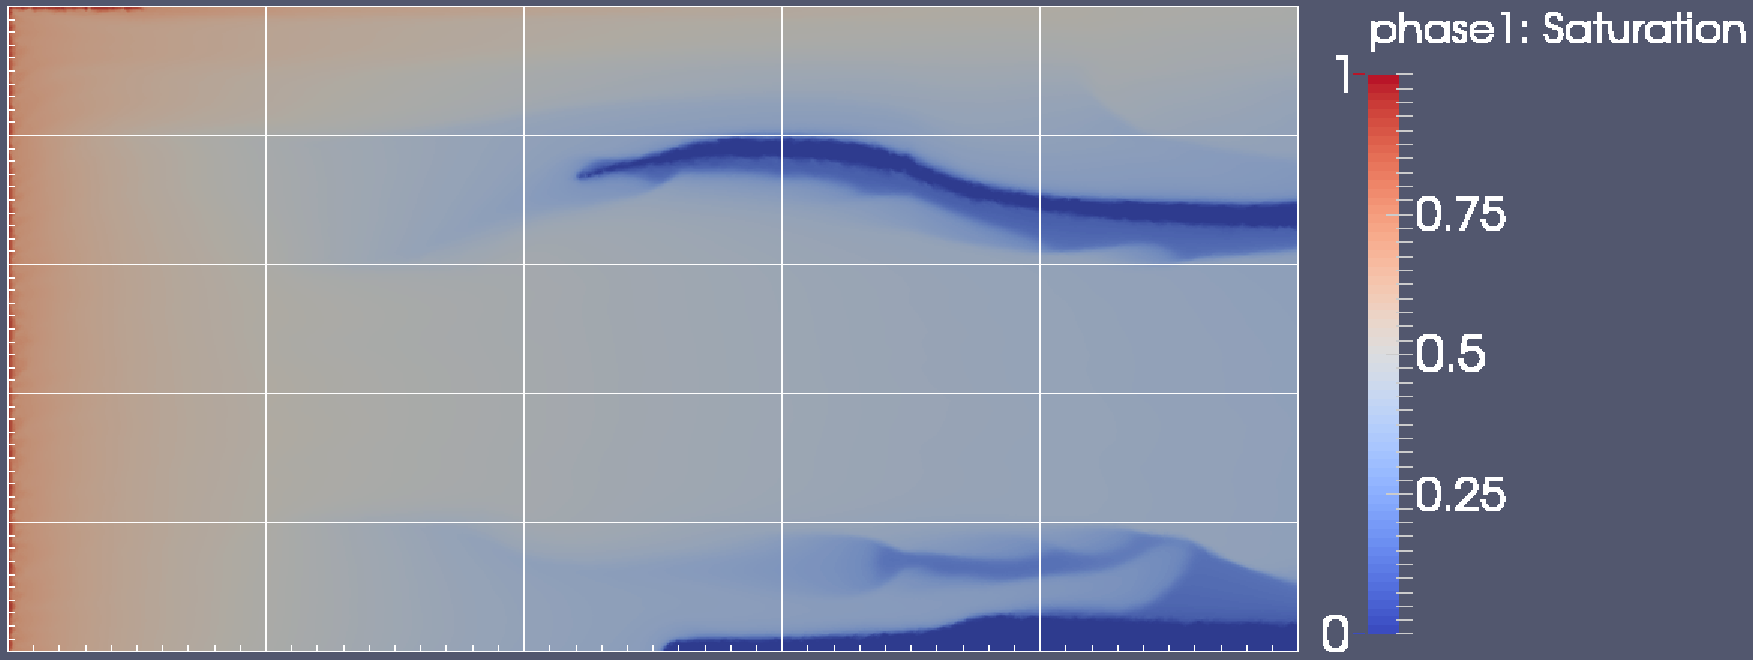
\includegraphics[width=.9\textwidth]{./Pics1/mr10_5regions_adapt/5regions_adapt_3000_1.pdf}
}
\vspace{0.0cm}
\hbox{\hspace{6.5cm} (b) flow at t=end (adaptive mesh)     
}
}     
\caption{Using the $P_{1}DGP_{2}$ element type for VR=$10$ under the same time steps, we compared the impact of fixed and adaptive mesh for the same timeframe. The end of simulation happens at $time=5 sec$ and for the timestemp $t=9999$ while the number of elements in both simulations was approximately $4700$. When adaptive mesh is introduce there is better repersentation of the fluid instabilities as these are developed on time.}
\label{fig:2testcase_d}
\end{figure}
\end{landscape}
\clearpage



%%%%
%%%%  FIGURE
%%%%
\begin{landscape}
\begin{figure}[ht] 
\vbox{
\hbox{\hspace{3.5cm}
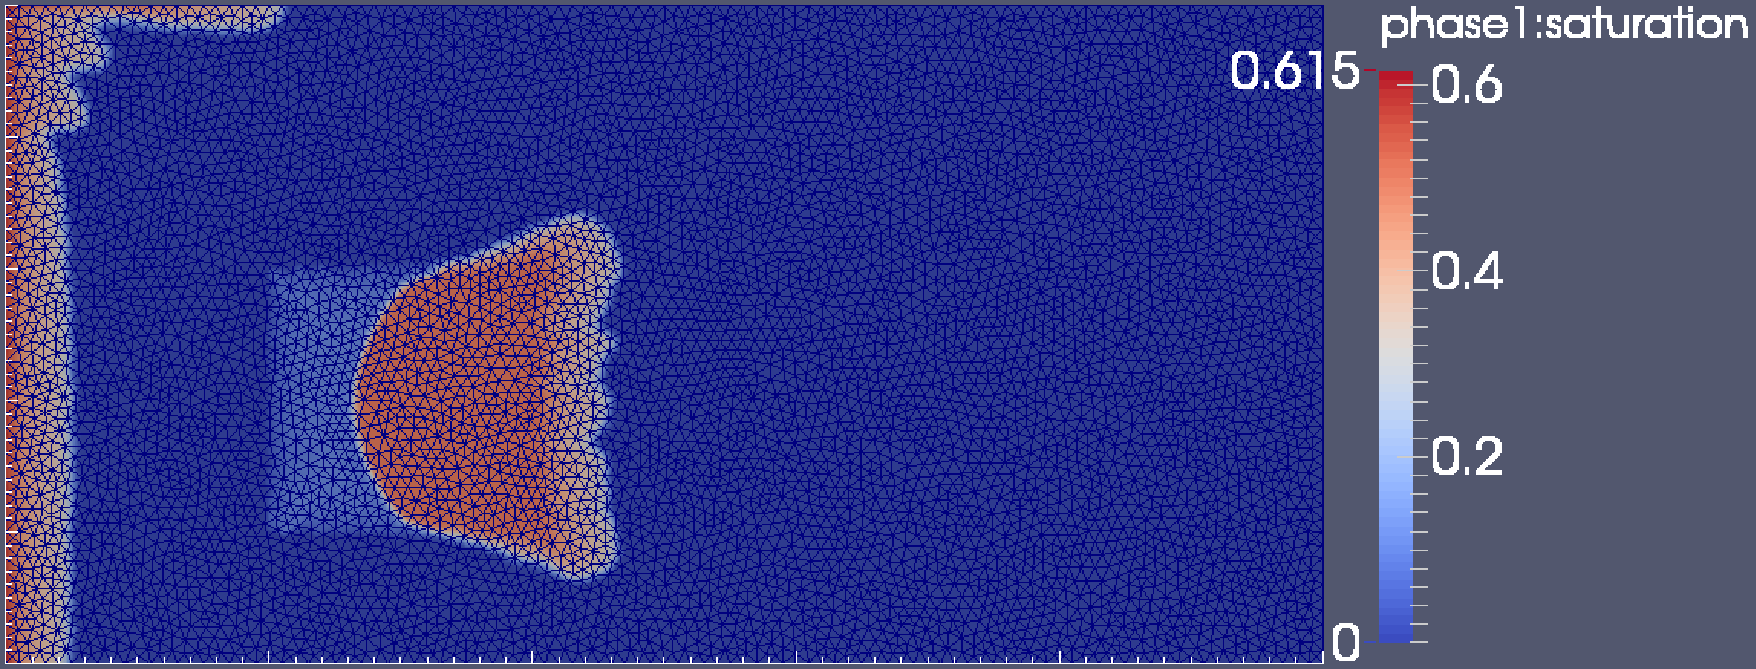
\includegraphics[width=.9\textwidth]{./Pics1/mr10_5regions_fixed_dinlet/5regions_dinlet_fixed_100_1.pdf}
}
\vspace{0.0cm}
\hbox{\hspace{6.5cm} (a) double inlet - fixed mesh   
}
\hbox{\hspace{3.5cm}
  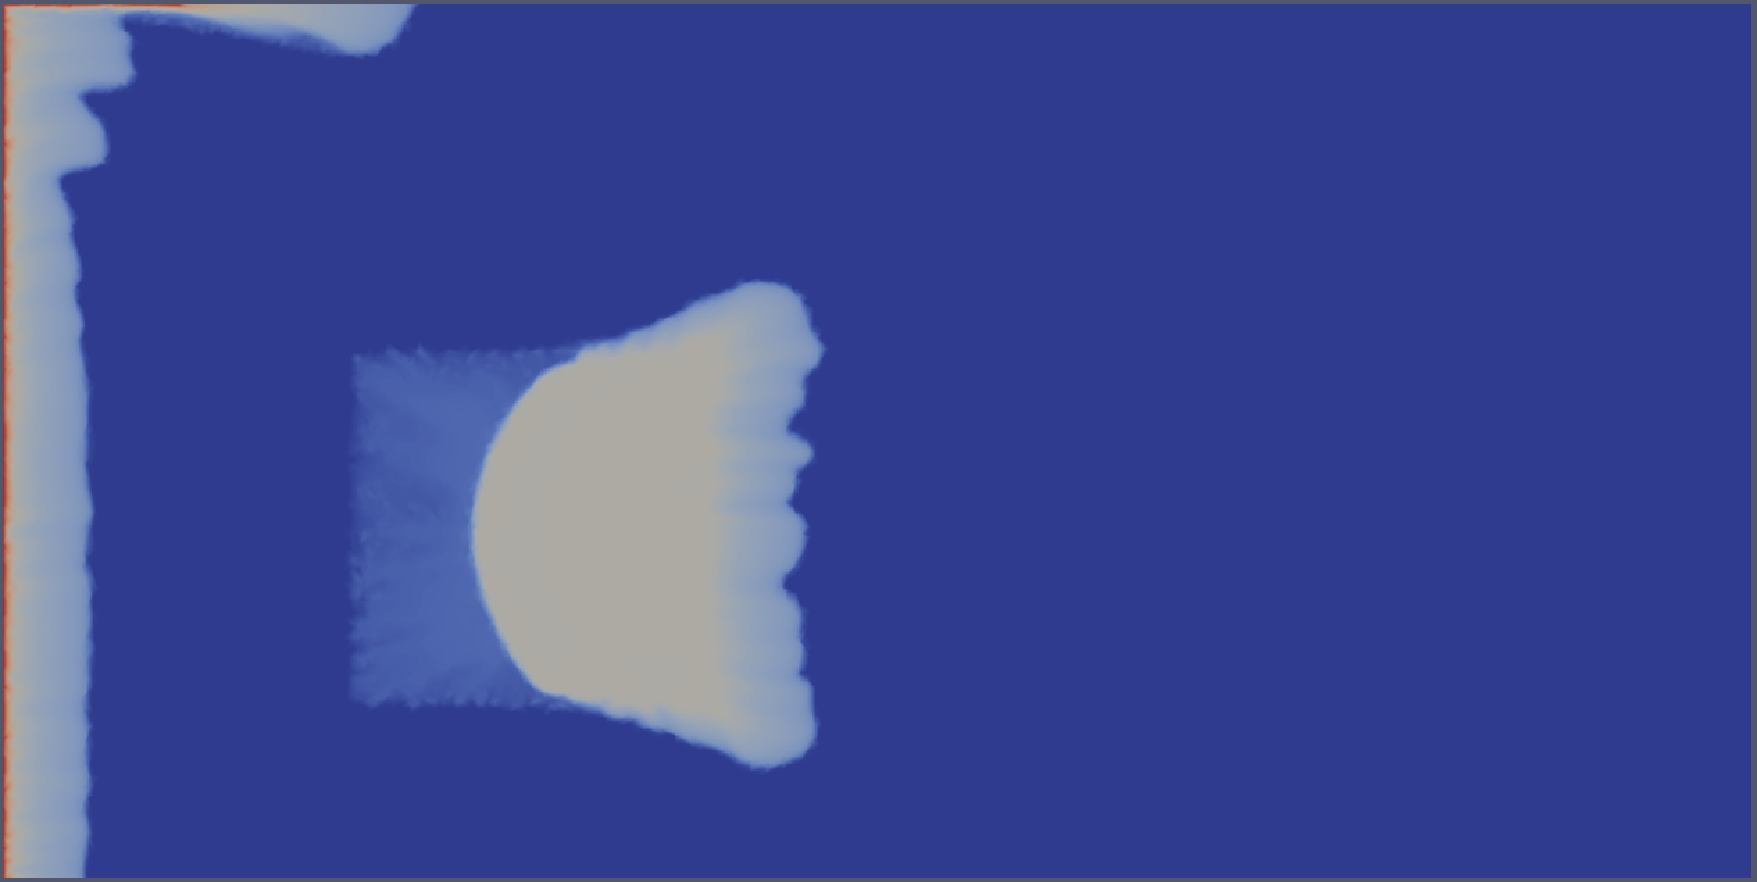
\includegraphics[width=.67\textwidth]{./Pics1/mr10_5regions_adapt_dinlet/5regions_dinlet_adapt_start.pdf}
}
\vspace{0.0cm}
\hbox{\hspace{6.5cm} (b) double inlet adaptive mesh   
}
}     
\caption{Comparing test-cases of fixed and adaptive mesh while a second region/inlet is introduced. For $t=0.101$s, using the $P_{1}DGP_{2}$ element type for MR=$10$ under the same time steps. For this simulation there are $13226$ elements for the fixed messh and $43716$ for the adaptive.}
\label{fig:3testcase_a}
\end{figure}
\end{landscape}
\clearpage

%%%%
%%%%  FIGURE
%%%%
\begin{figure}[ht] 
\vbox{
\hbox{\hspace{3.5cm}
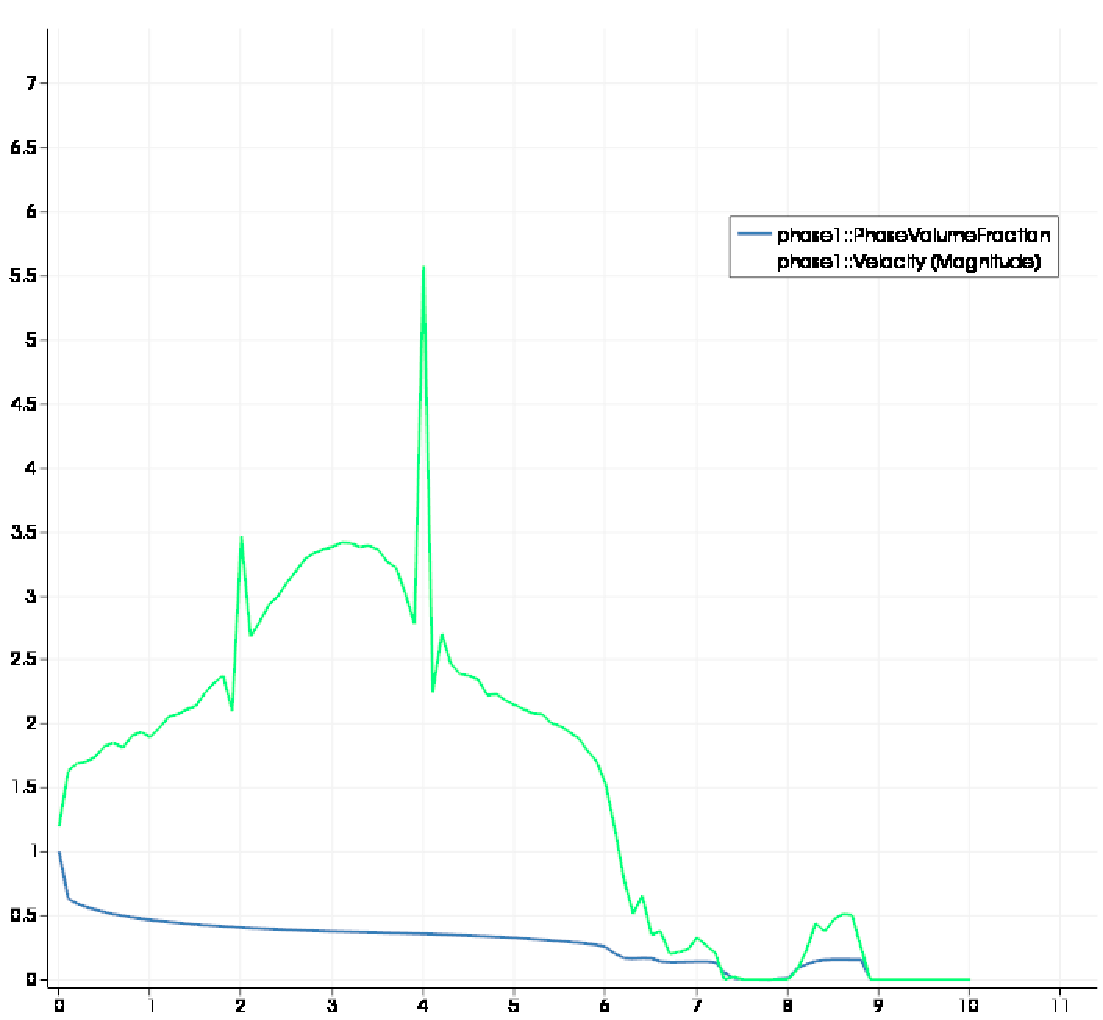
\includegraphics[width=.5\textwidth]{./Pics1/mr10_5regions_adapt/5regions_adapt_vel_magn.pdf} 
}
\vspace{0.0cm}
\hbox{\hspace{5.0cm} (a) single inlet velocity magnitude   
}
\hbox{\hspace{3.5cm}
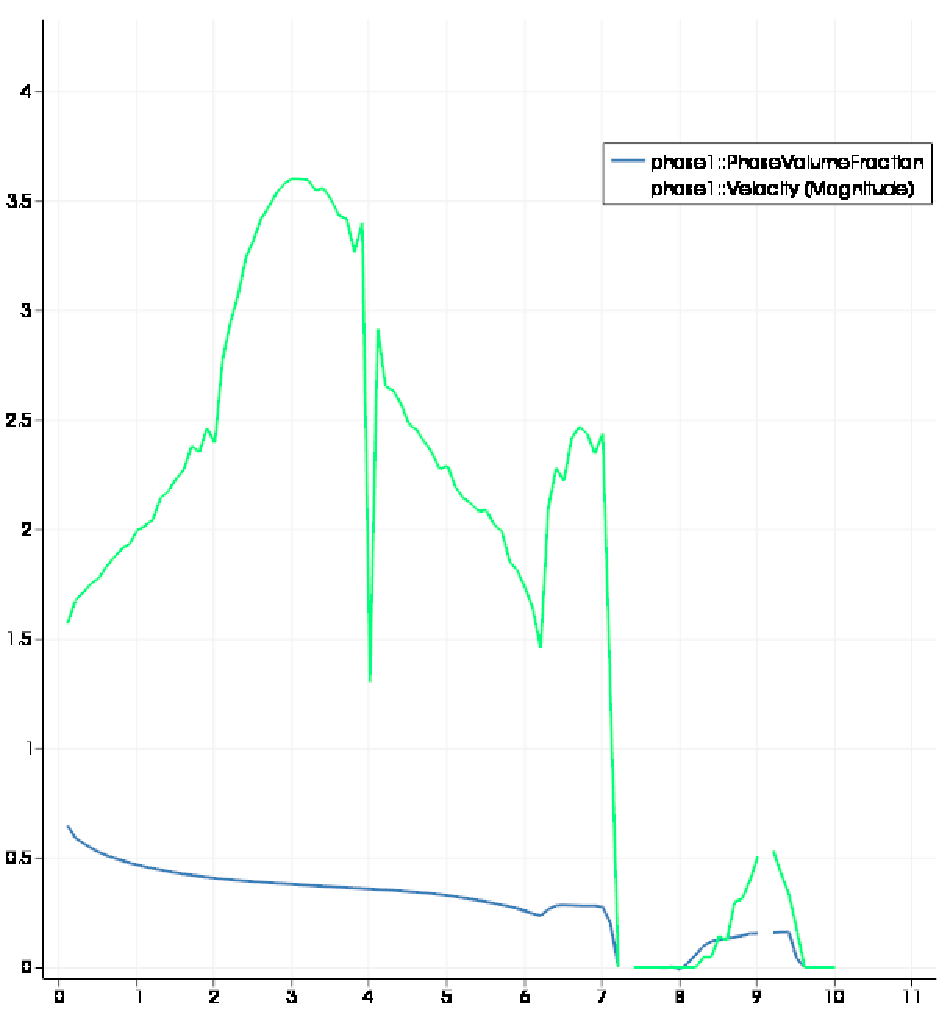
\includegraphics[width=.5\textwidth]{./Pics1/mr10_5regions_adapt_dinlet/5regions_dinlet_adapt_vel_magn.pdf}
}
\vspace{0.0cm}
\hbox{\hspace{5.0cm} (b) double inlet velocity magnitude   
}
}     
\caption{For the same time step, t=1000, these plots describe the velocity magnitudes of the phase $1$ (injected fluid) under the same boundary and initiall conditions. From top to bottom,these graphs describe the velocity magnitude %for fixed mesh is plotted(top), the velocity magnitude 
for adaptive mesh-single inlet (top) and the velocity magnitude for adaptive mesh with double inlet (bottom) as these are also presented in fig.\ref{fig:3testcase_a}. The main difference between the upper and lower plot %is not just the ability to capture in greater detail, the fluid instabilities as they happenduring the finger development and their velocity patterns. While there 
is the impact of the second injection interval as this can be seen from the slope and the rate that the velocity magnitude is changing.}
\label{fig:vel_magn}
\end{figure}

%%%%
%%%%  FIGURE
%%%%
\begin{landscape}
\begin{figure}[ht] 
\vbox{
\hbox{\hspace{3.5cm}
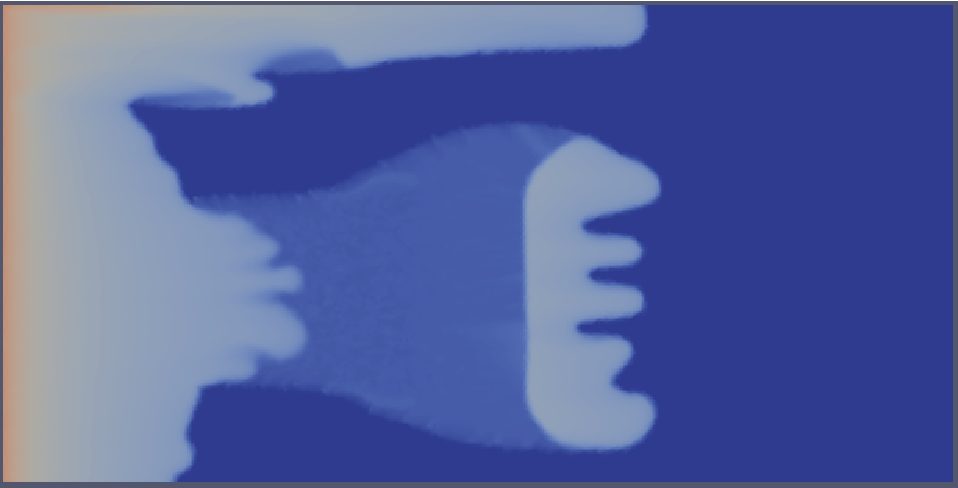
\includegraphics[width=.65\textwidth]{./Pics1/5reg_dinlet_fixed_500.pdf} 
}
\vspace{0.0cm}
\hbox{\hspace{6.5cm} (a) double inlet - fixed mesh   
}
\hbox{\hspace{3.5cm}
\includegraphics[width=.9\textwidth]{./Pics1/5reg_dinlet_adapt_500_1.pdf}
}
\vspace{0.0cm}
\hbox{\hspace{6.5cm} (b) double inlet adaptive mesh   
}
}     
\caption{For $t=5$s there is a comparison between fixed mesh(a) and adaptive mesh(b).}
\label{fig:3testcase_b}
\end{figure}
\end{landscape}
\clearpage

%%%%
%%%%  FIGURE
%%%%
\begin{landscape}
\begin{figure}[ht] 
\vbox{
\hbox{\hspace{3.5cm}
\includegraphics[width=.65\textwidth]{./Pics1/5reg_dinlet_fixed_1500.pdf} 
}
\vspace{0.0cm}
\hbox{\hspace{6.5cm} (a) double inlet - fixed mesh   
}
\hbox{\hspace{3.5cm}
\includegraphics[width=.9\textwidth]{./Pics1/5reg_dinlet_adapt_1500_1.pdf}
}
\vspace{0.0cm}
\hbox{\hspace{6.5cm} (b) double inlet adaptive mesh   
}
}     
\caption{For $t=7.5$s this is a comparison between fixed mesh(a) and adaptive mesh(b).}
\label{fig:3testcase_c}
\end{figure}
\end{landscape}
\clearpage

%%%%
%%%%  FIGURE
%%%%
\begin{landscape}
\begin{figure}[ht] 
\vbox{
\hbox{\hspace{3.5cm}
\includegraphics[width=.65\textwidth]{./Pics1/5reg_dinlet_fixed_end.pdf} 
}
\vspace{0.0cm}
\hbox{\hspace{6.5cm} (a) double inlet - fixed mesh   
}
\hbox{\hspace{3.5cm}
\includegraphics[width=.9\textwidth]{./Pics1/5reg_dinlet_adapt_end_1.pdf}
}
\vspace{0.0cm}
\hbox{\hspace{6.5cm} (b) double inlet adaptive mesh   
}
}     
\caption{This is a comparison between fixed mesh(a) and adaptive mesh(b) at the end of the simulation. For the fixed mesh at this point the maximum number of point is $13226$ while for the adaptive mesh is $7582$ and most of them are located where is needed in the domain.}
\label{fig:3testcase_d}
\end{figure}
\end{landscape}
\clearpage

%%%%
%%%%  FIGURE
%%%%
\begin{landscape}
\begin{figure}[ht] 
\vbox{
\hbox{\hspace{3.5cm}
\includegraphics[width=.8\textwidth]{./Pics1/mr100_fixed/mr100_fixed_500.pdf} 
}
\vspace{0.0cm}
\hbox{\hspace{4.0cm} (a) fixed and unstructured mesh for MR = 100 (start)   
}
\hbox{\hspace{3.5cm}
\includegraphics[width=.8\textwidth]{./Pics1/mr100_fixed/mr100_fixed_1500.pdf}
}
\vspace{0.0cm}
\hbox{\hspace{3.75cm} (b) fixed and unstructured mesh for MR = 100 (t = 1500)   
}
}     
\caption{For the case of VR=$100$ from top to bottom, the number of elements is $4680$ and fixed and unstructured mesh for the same time steps, t=$0.25$ or t=500(a), t=$0.75$ or t=1500(b). }
\label{fig:4testcase_a}
\end{figure}
\end{landscape}
\clearpage

%%%%
%%%%  FIGURE
%%%%
\begin{landscape}
\begin{figure}[ht] 
\vbox{
\hbox{\hspace{3.5cm}
\includegraphics[width=.8\textwidth]{./Pics1/mr100_fixed/mr100_fixed_3000.pdf} 
}
\vspace{0.0cm}
\hbox{\hspace{3.75cm} (c) fixed and unstructured mesh for MR = 100    
}
\hbox{\hspace{3.5cm}
\includegraphics[width=.8\textwidth]{./Pics1/mr100_fixed/mr100_fixed_end.pdf}
}
\vspace{0.0cm}
\hbox{\hspace{7.cm} (d) end of simulations     
}
}     
\caption{screenshot (c) is for t=$1.5$ sec or t=$3000$ and screenshot (d) is for t=$3.175$ sec, at the end of the simulations. }
\label{fig:4testcase_b}
\end{figure}
\end{landscape}
\clearpage



%

%%%
%%%  FIGURE 
%%%
\begin{figure}[h]
\begin{center}
\includegraphics[width=1.\textwidth]{diagrams/bl-exact-meth-upwind.eps}
\end{center}
\caption{Buckley--Leverett test-cases: Saturation solutions for the continuous upwind method for different 1D P$_{1}$DG-P$_{2}$ mesh  resolutions and comparison against standard analytical solution.
\label{bl-exact-meth-upwind}}
\end{figure}

%%%
%%%
%%%  FIGURE 
%%%
\begin{figure}[h]
  %\begin{center}
\vbox{\hbox{\hspace{2.5cm}
    \includegraphics[width=0.62\textwidth]{diagrams/BL_1d_P0DGP1_convergence.eps}}
\vspace{-.0cm}\hbox{\hspace{2.5cm}
    \includegraphics[width=0.62\textwidth]{diagrams/BL_1d_P1DGP2_convergence.eps}}
\vspace{-.0cm}\hbox{\hspace{2.5cm}
    \includegraphics[width=0.62\textwidth]{diagrams/BL_1d_P2DGP3_convergence.eps}}}
   % \includegraphics[width=0.45\textwidth]{BL_2d_P1DGP2_convergence}
    \caption{Buckley--Leverett test-cases: Saturation profiles for a number of element-pairs and numerical resolutions in 1D -- P$_{0}$DG-P$_{1}$ (top), P$_{1}$DG-P$_{2}$ and P$_{2}$DG-P$_{3}$ (bottom).\label{fig:BL_profiles}}
  %\end{center}
\end{figure}

%%%
%%%  FIGURE 
%%%
\begin{figure}[h]
\vbox{\hbox{\hspace{1.cm}
    \includegraphics[width=0.8\textwidth]{diagrams/L1_convergence_rate.eps}}
\vspace{.0cm}\hbox{\hspace{1.cm}
    \includegraphics[width=0.8\textwidth]{diagrams/L2_convergence_rate.eps}}}
    \caption{Buckley--Leverett test-cases: L1 (top) and L2 (bottom) error convergence rates for a number of element pairs. \label{fig:BL_converg-rates}}
\end{figure}

%%%
%%%  FIGURE 
%%%
\begin{figure}[h]
\begin{center}
\includegraphics[width=1.\textwidth]{diagrams/bl-upwind-v-up-and-down.eps}
\end{center}
\caption{Buckley--Leverett test-cases: Comparison of the optimal upwind formulation when using upwinding (OU) and coupled upwind/downwind (OU-D). The finite element interpolation of the saturation field $\left(S_{1}\right)$ is shown at different mesh resolutions. Downwind seems to detract from the accuracy of the solution. \label{bl-upwind-v-up-and-down}}
\end{figure}

%%%
%%%  FIGURE 
%%%
\begin{figure}[h]
\vbox{
\begin{center}
\includegraphics[width=1.\textwidth]{diagrams/bl-exact-meth-cv-0-8-ele50.eps}
\end{center}
\vspace{0.cm}}
\caption{Buckley--Leverett test-cases: Comparison of control volume
  solutions using 80$\%$ upwinding and with optimal upwinding and
  using 50 continuous P$_{1}$DG-P$_{2}$
  elements. \label{bl-exact-meth-cv-0-8-ele50}}
\end{figure}

%%%
%%%  FIGURE 
%%%
\begin{figure}[h]
\begin{center}
\includegraphics[width=1.\textwidth]{diagrams/bl-dg-2eles.eps}
\end{center}
\caption{Buckley--Leverett test-cases: Two element solution using the
  discontinuous formulation. Saturation field from both CV solution
  and FEM interpolation are shown.  \label{bl-dg-2eles}}
\end{figure}

%%%
%%%  FIGURE 
%%%
\begin{figure}[h]
\vbox{
\hbox{\hspace{.3cm}\includegraphics[width=.9\textwidth]{diagrams/bl-dg-4-10-20.eps}}
\vspace{-0.cm}
\hbox{\hspace{.3cm}\includegraphics[width=.9\textwidth]{diagrams/bl-dg-cent-4-10-20.eps}}}
\caption{Buckley--Leverett test-cases: Saturation field obtained from
  the discontinuous and continuous formulation with different mesh
  resolutions. Solutions with (top) and without (bottom) upwinding
  scheme. Notice that oscillations are suppressed with the upwinding
  scheme.\label{bl-dg-cent-4-10-20}}
\end{figure}


%%%
%%%  FIGURE 
%%%
\begin{figure}[h]
\vbox{
\hbox{\hspace{.3cm}\includegraphics[width=.9\textwidth]{diagrams/bl-dg-4-10-vers-cty.eps}}
\vspace{-0.cm}
\hbox{\hspace{.3cm}\includegraphics[width=.9\textwidth]{diagrams/bl-dg-p1-2-4-5-10-20-40.eps}}}
\caption{Buckley--Leverett test-cases: Saturation field obtained from
  (top) continuous and discontinuous (between elements) formulations
  (solution with 50 elements may be considered as a converged
  result). Solution obtained (bottom) from linear pressure (P1)
  formulation with different mesh resolution with comparison against
  P2-pressure formulation (continuous). \label{bl-dg-4-10-vers-cty}}
\end{figure}


%%%
%%%  FIGURE 
%%%
\begin{figure}[H]
\vbox{
\begin{center}
\includegraphics[width=17.5cm,height=12.5cm]{diagrams/bl-dg-4-10-vers-cty}
\end{center}
\vspace{0.cm}}
\caption{Gas saturations shown comparing the accuracy of the
  discontinuous between elements and continuous formulation. The 50
  element continuous solution may be viewed as a converged result.  }
\label{bl-dg-4-10-vers-cty}
\end{figure}

\begin{comment}
%%%
%%%  FIGURE 
%%%
\begin{figure}[h]
\vbox{
\hbox{\hspace{.2cm}
    \includegraphics[width=1.\textwidth]{diagrams/map_2d.png}}
\vspace{1.cm}
\hbox{\hspace{0.2cm}
    \includegraphics[width=1.\textwidth]{./diagrams/map_3d.png}}}
    \caption{Buckley-Leverett test-cases: phase 1 saturation surface maps for a 2- (770 triangles) and 3-D (1207 tetrahedra) simulations (\PN[1]{2} unstructured mesh grids) at time $t=0.5$. \label{fig:maps2d_3d}}
\end{figure}


%%%  FIGURE 
%%%
\begin{figure}[h]
\vbox{\hbox{\hspace{.3cm}
    \includegraphics[width=0.9\textwidth]{diagrams/BL_2d_P1DGP2_convergence.eps}}
\vspace{-.0cm}\hbox{\hspace{.3cm}
    \includegraphics[width=0.9\textwidth]{./diagrams/simulations_2d_3d.eps}}}
    \caption{Buckley-Leverett test-cases: 2- and 3-D phase 1 saturation profiles with \PN[1]{2} elements. Sensitivity analysis for (top) grid resolution using structured \PN[1]{2} mesh, and (bottom) mesh type.\label{fig:BL_2d_profiles}}
\end{figure}

\end{comment}
 

\end{document}
%% End of tex file.


